\section{Resultados}
En esta sección incluiremos los resultados de la experimentación que realizamos con las redes desarrolladas.\\

La idea general de los experimentos es intentar medir la performance
de cada red observando, en el primer problema, la distribución espacial de los clusters de empresas y en el segundo, la calidad 
del mapa generado y la capacidad de generalizar.

A lo largo de los ejercicios, dividimos el dataset en dos conjuntos: entrenamiento y validación. El primero contiene al 90\% de los datos, elegidos
azarosa y uniformemente en relacion a categoría. El resto de los documentos se agruparon para validar los resultados obtenidos en el entrenamiento.

Presentamos en primer lugar los resultados obtenidos del problema de reducción de dimensiones.

\subsection{Ejercicio 1 - Reducción de dimensiones}

Para el primer ejercicio, los experimentos consistieron en variar la cantidad de épocas, la regla de aprendizaje y la cantidad de dimensiones de salida. Intentamos variar estos factores y observar diferencias en los gráficos 3D generados en base a las nuevas dimensiones.

Comenzamos realizando clasificaciones con 100 épocas. Al obtener resultados imprecisos subimos la cantidad a 200. Allí observamos una clasificación mejor, más marcada la separación geométrica entre los distintos clusters.

Luego comparamos los resultados obtenidos entre las distintas reglas. Repetimos las ejecuciones variando la regla entre Oja y Sanger para comprobar su eficacia.

Por último, decidimos cambiar la cantidad de dimensiones de sálida, esperando una mejora en las clasificaciones. 

\subsubsection{Regla de Oja - variando número de épocas}
En los primeros experimentos, fuimos probando la calidad de la clasificación utilizando solamente 100 épocas. La decisión se basó en un tema de performance de la red. Cada ejecución tenía una considerable demora, por lo que empezamos probando con pocas épocas. Mostramos los primeros resultados que obtuvimos, utilizando la regla de Oja:

\begin{figure}[!htbp]
\centering
\begin{subfigure}{.5\textwidth}
  \centering
  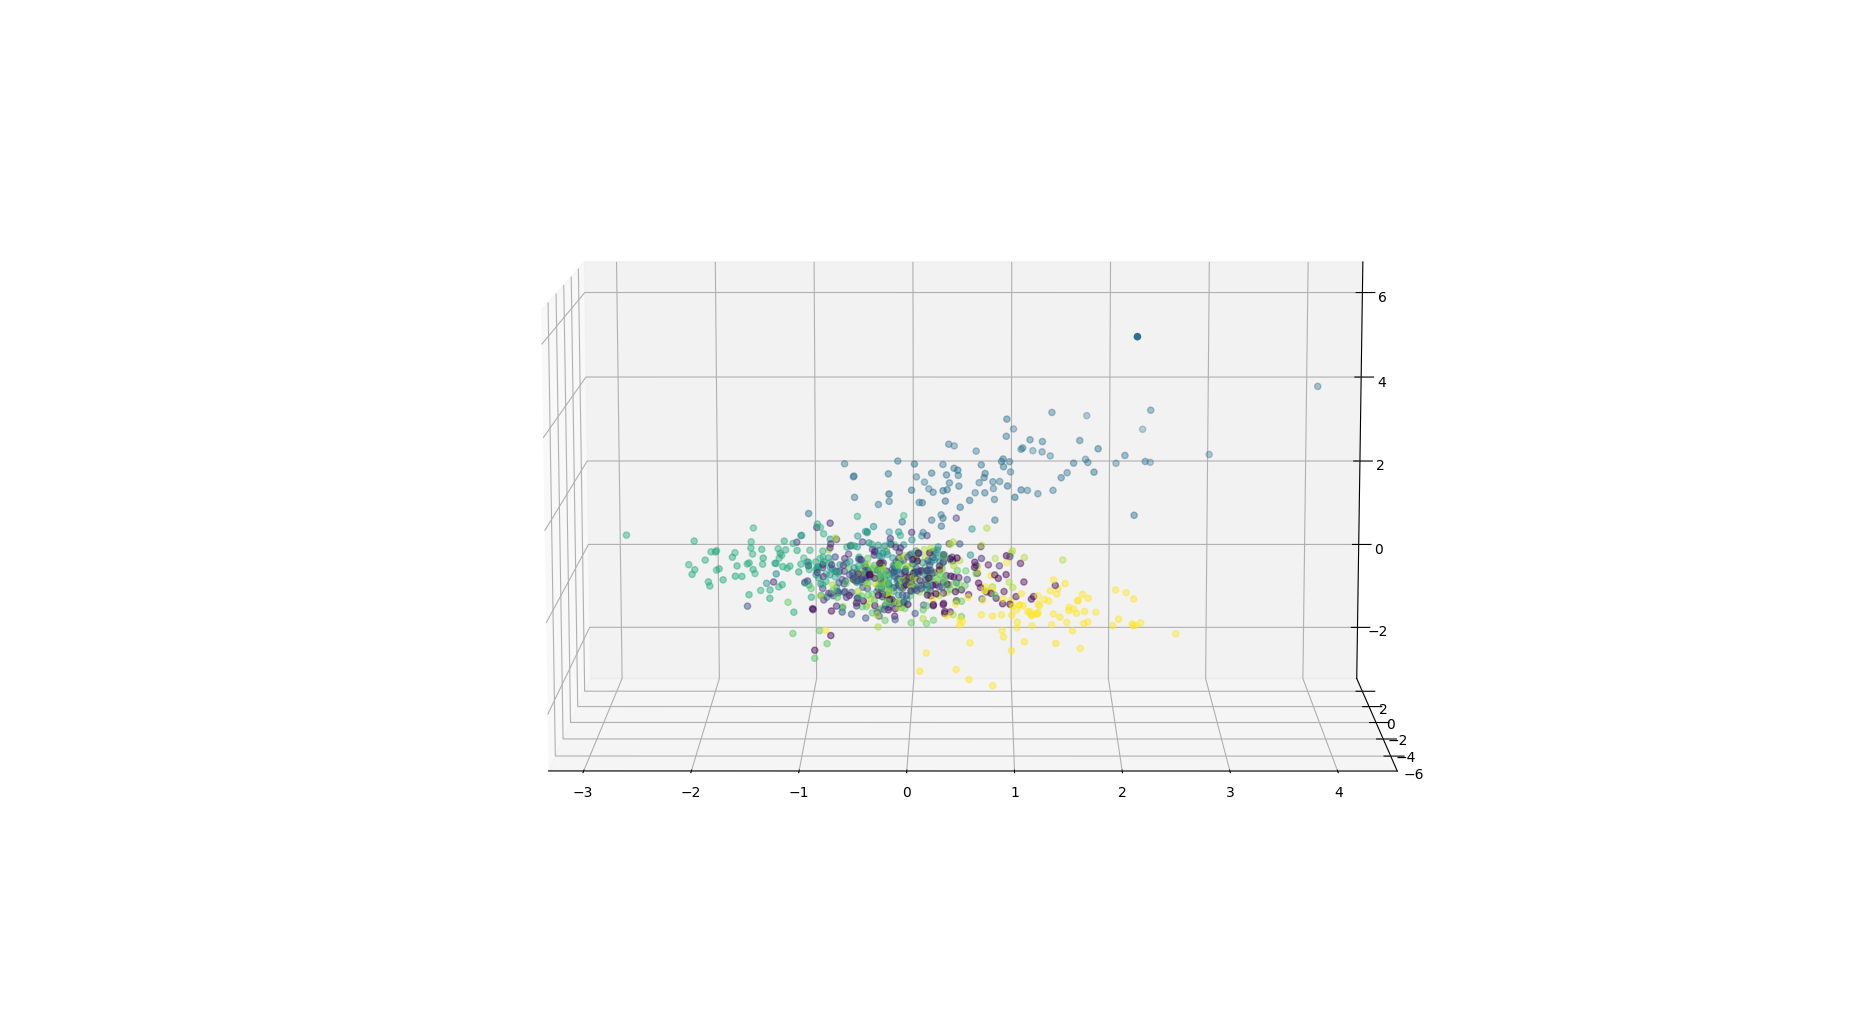
\includegraphics[width=1\linewidth, scale=1]{../img/ej1/oja/oja_3salida_100ep_train_2.png}
  \caption{Oja - 3 dimensiones - 100 épocas}
  \label{fig:sub1}
\end{subfigure}%
\begin{subfigure}{.5\textwidth}
  \centering
  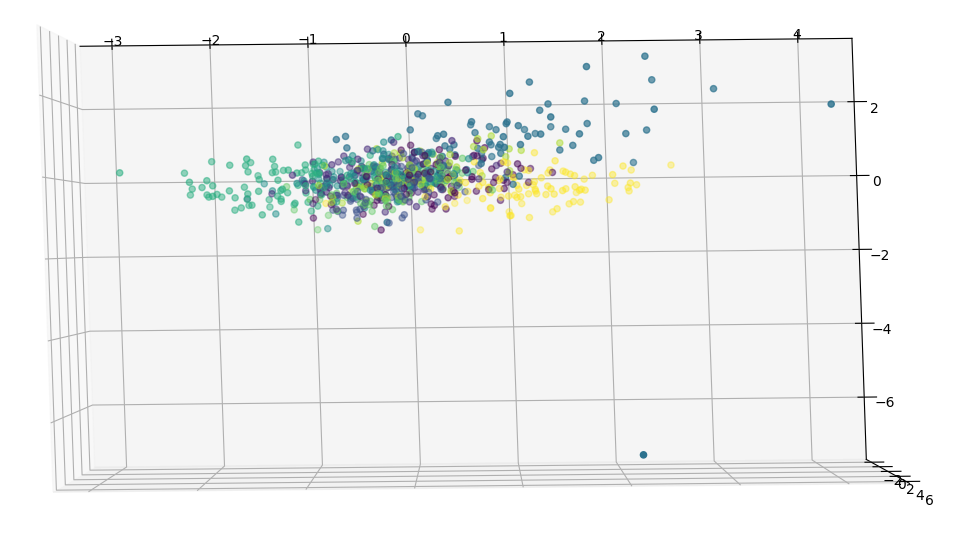
\includegraphics[width=1\linewidth, scale=1]{../img/ej1/oja/oja_3salida_100ep_train_3.png}
  \caption{Oja - 3 dimensiones - 100 épocas}
  \label{fig:sub2}
\end{subfigure}
\end{figure}

\newpage

\begin{figure}[h]
  \begin{center}
    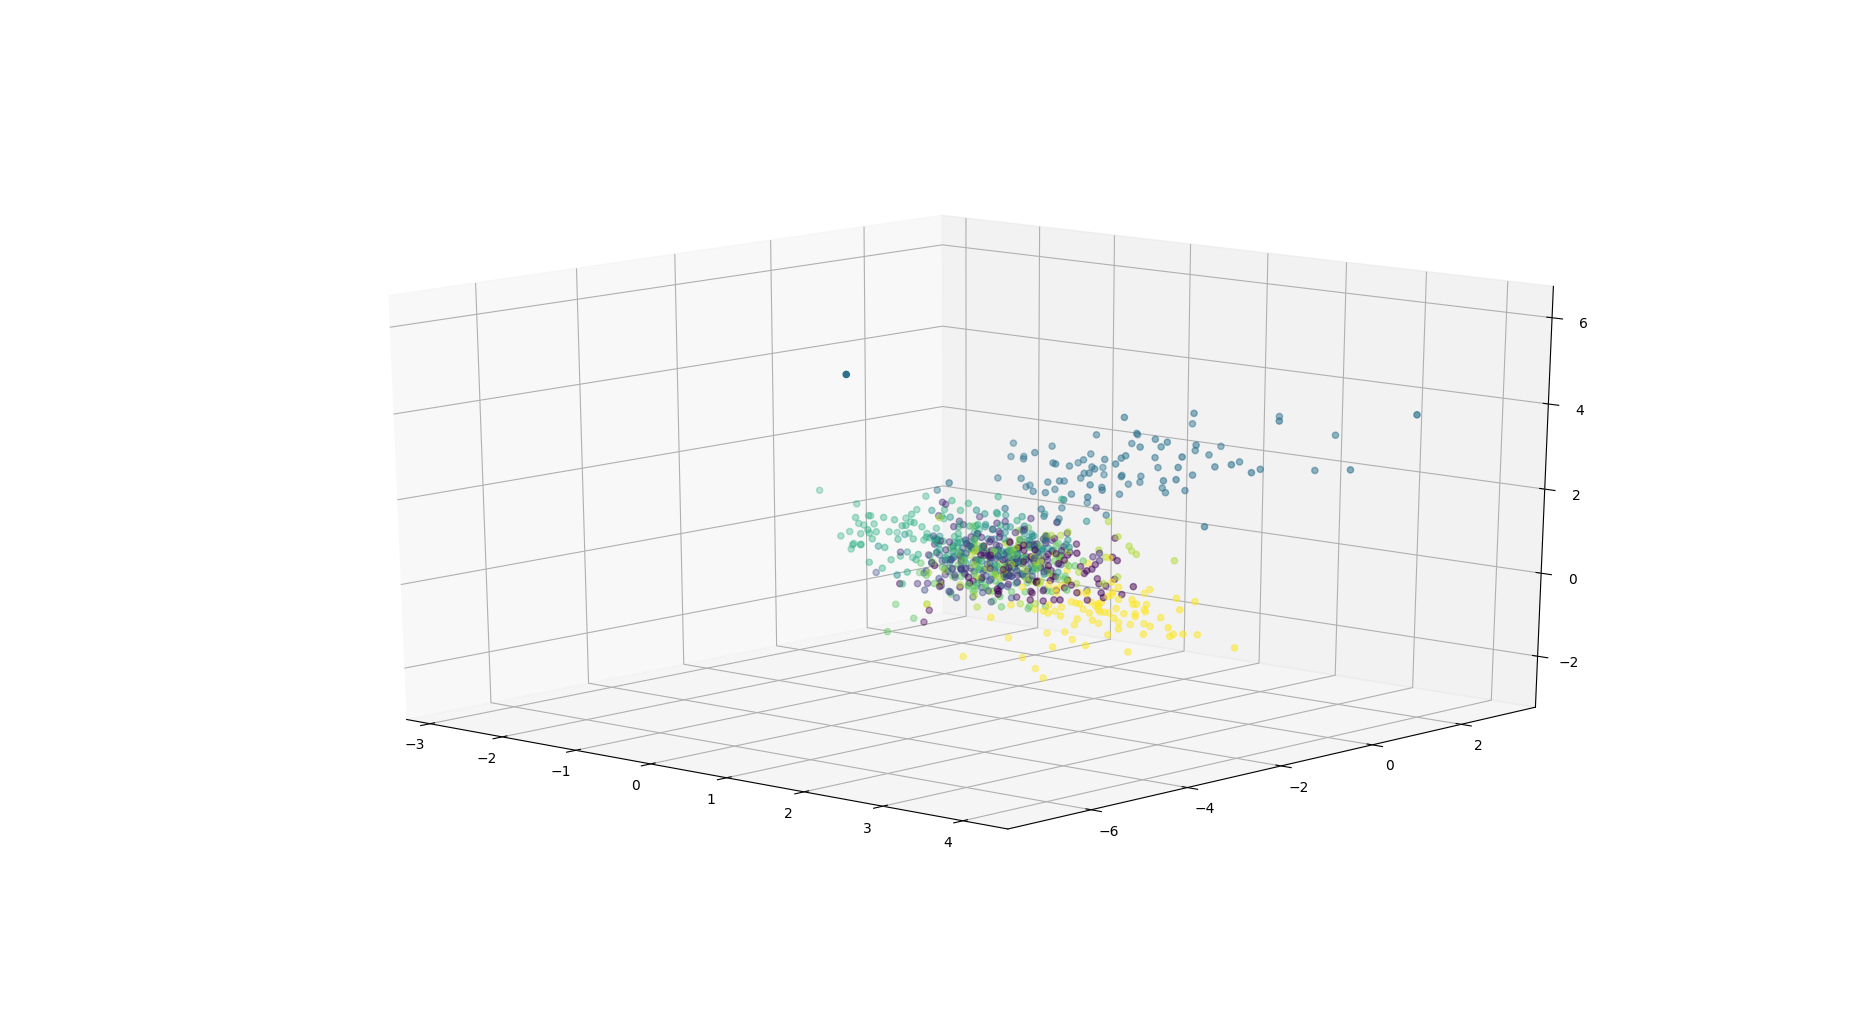
\includegraphics[scale=0.45]{../img/ej1/oja/oja_3salida_100ep_train.png}
  \caption{Oja - 3 dimensiones - 100 épocas - Datos Entrenamiento}
  \end{center}
\end{figure}

Éstos son los gráficos de las ejecuciones utilizando regla de Oja, con 100 épocas. Notamos que se están comenzando a formar
clusters de clasificación con distintos colores, pero que también hay mucho solapamiento en la parte central de cada vista.\\

Luego de esta etapa de entrenamiento, procesamos los datos de validación:

\begin{figure}[!htbp]
\centering
\begin{subfigure}{.5\textwidth}
  \centering
  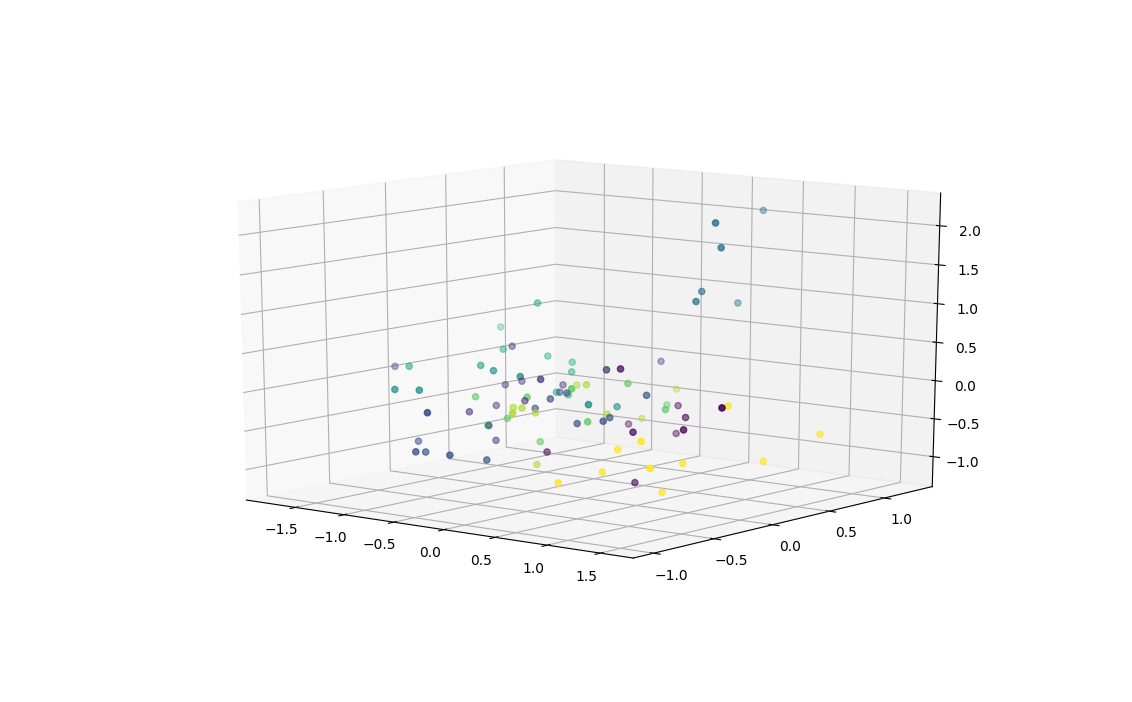
\includegraphics[width=1\linewidth, scale=1]{../img/ej1/oja/oja_3salida_100ep_validation.png}
  \caption{Oja - 3 dimensiones - 100 épocas}
  \label{fig:sub1}
\end{subfigure}%
\begin{subfigure}{.5\textwidth}
  \centering
  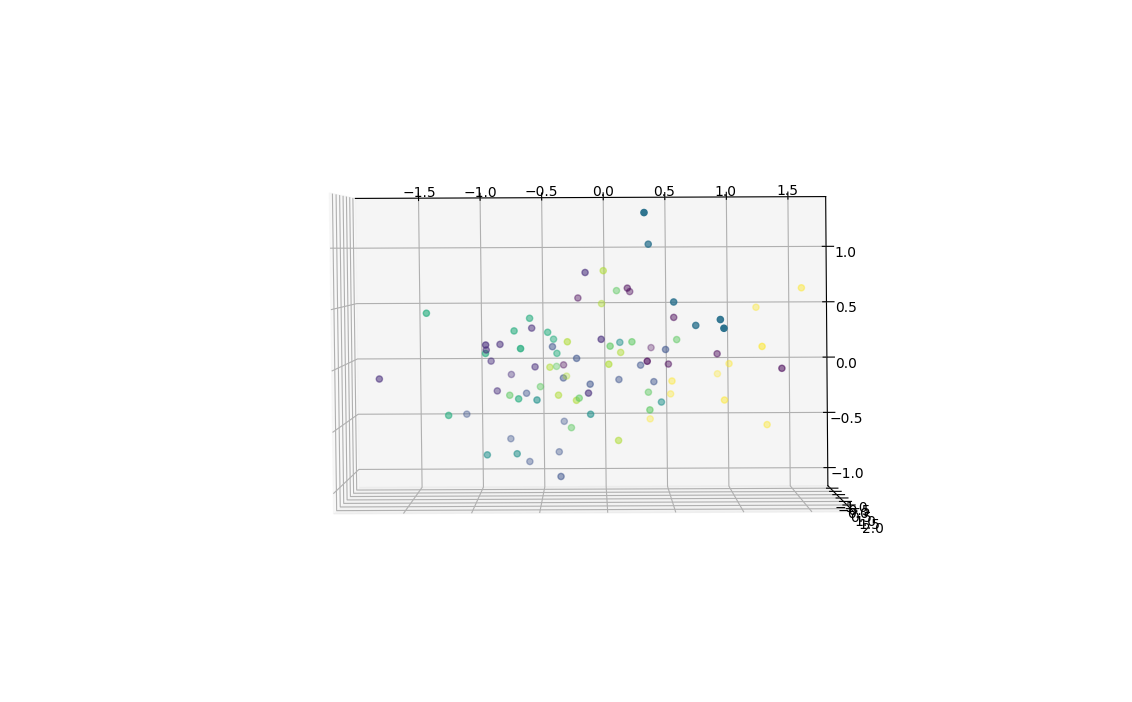
\includegraphics[width=1\linewidth, scale=1]{../img/ej1/oja/oja_3salida_100ep_validation_3.png}
  \caption{Oja - 3 dimensiones - 100 épocas}
  \label{fig:sub2}
\end{subfigure}
\end{figure}

\begin{figure}[h]
  \begin{center}
    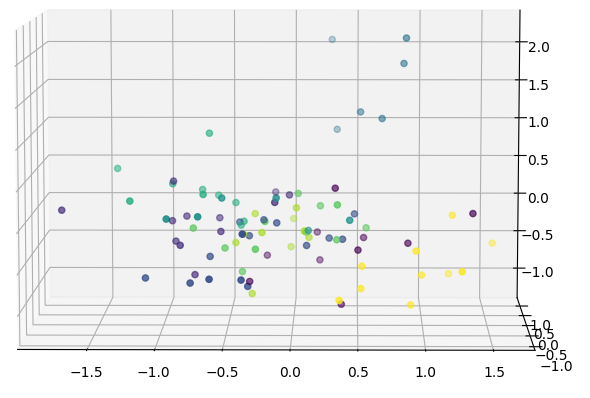
\includegraphics[scale=0.65]{../img/ej1/oja/oja_3salida_100ep_validation_2.png}
  \caption{Oja - 3 dimensiones - 100 épocas - Datos Validación}
  \end{center}
\end{figure}

\newpage

Para los datos de validación vemos una dispersión muy grande. Se notan algunos puntos del mismo color agrupados levemente cerca, pero lejos
de formar una división clara.\\

Luego de obtener estos resultados, menos precisos de lo que esperábamos, decidimos intentar probar subiendo número de épocas. Observemos a continuación las mismas ejecuciones, pero subiendo el número de épocas a 200:

\begin{figure}[!htbp]
\centering
\begin{subfigure}{.5\textwidth}
  \centering
  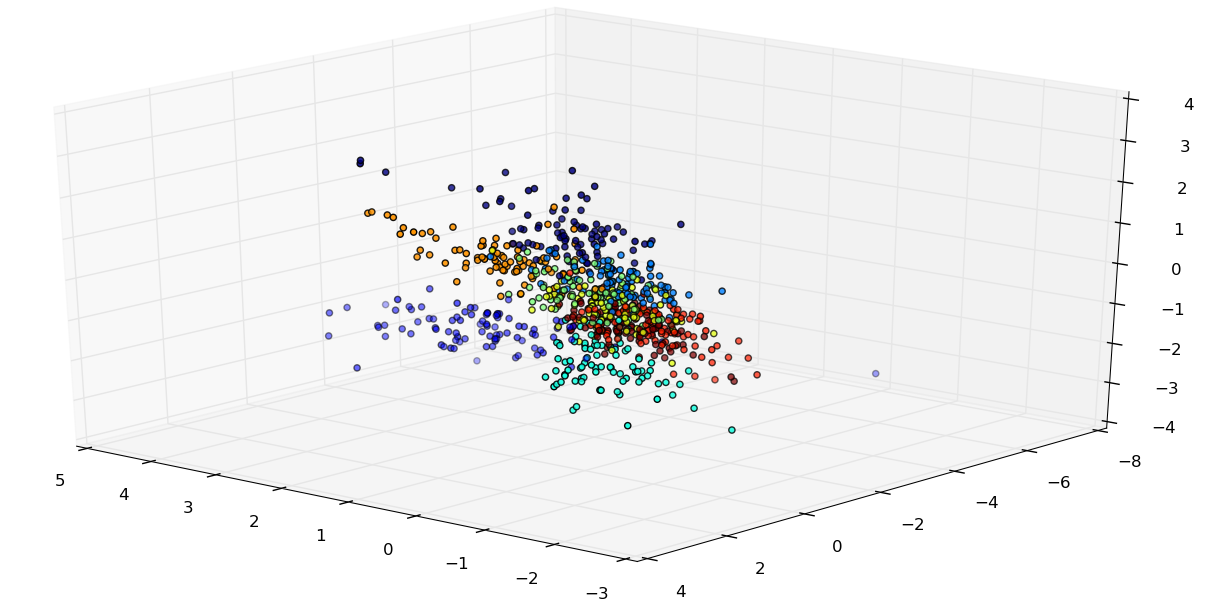
\includegraphics[width=1\linewidth, scale=1]{../img/ej1/oja/oja_3salida_200ep_train.png}
  \caption{Oja - 3 dimensiones - 200 épocas}
  \label{fig:sub1}
\end{subfigure}%
\begin{subfigure}{.5\textwidth}
  \centering
  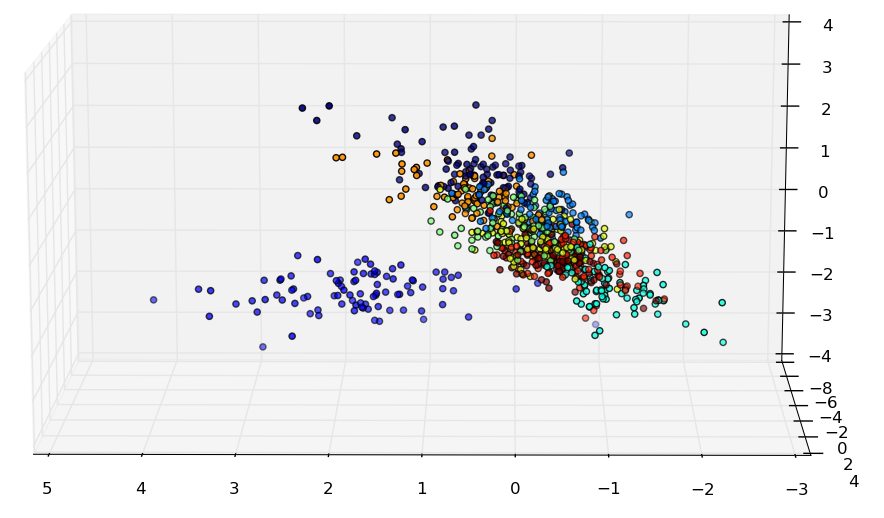
\includegraphics[width=1\linewidth, scale=1]{../img/ej1/oja/oja_3salida_200ep_train_2.png}
  \caption{Oja - 3 dimensiones - 200 épocas}
  \label{fig:sub2}
\end{subfigure}
\end{figure}
\begin{figure}[!htbp]
\centering
\begin{subfigure}{.5\textwidth}
  \centering
  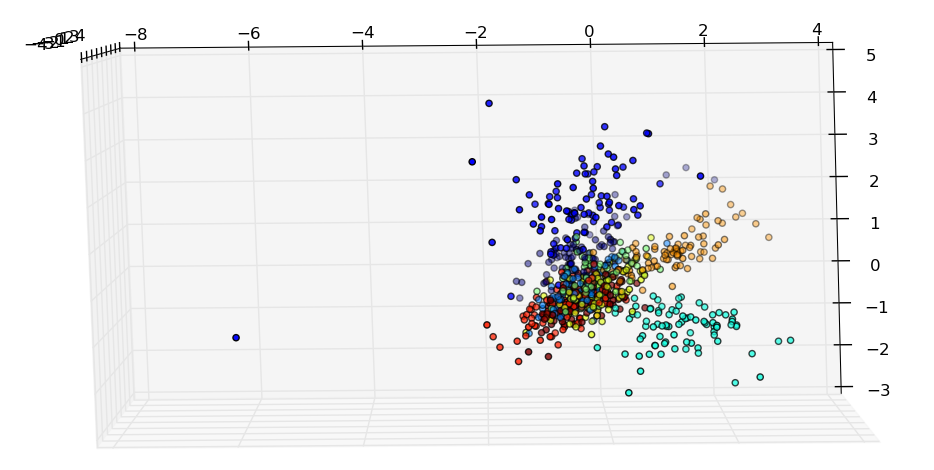
\includegraphics[width=1\linewidth, scale=1]{../img/ej1/oja/oja_3salida_200ep_train_3.png}
  \caption{Oja - 3 dimensiones - 200 épocas}
  \label{fig:sub3}
\end{subfigure}%
\begin{subfigure}{.5\textwidth}
  \centering
  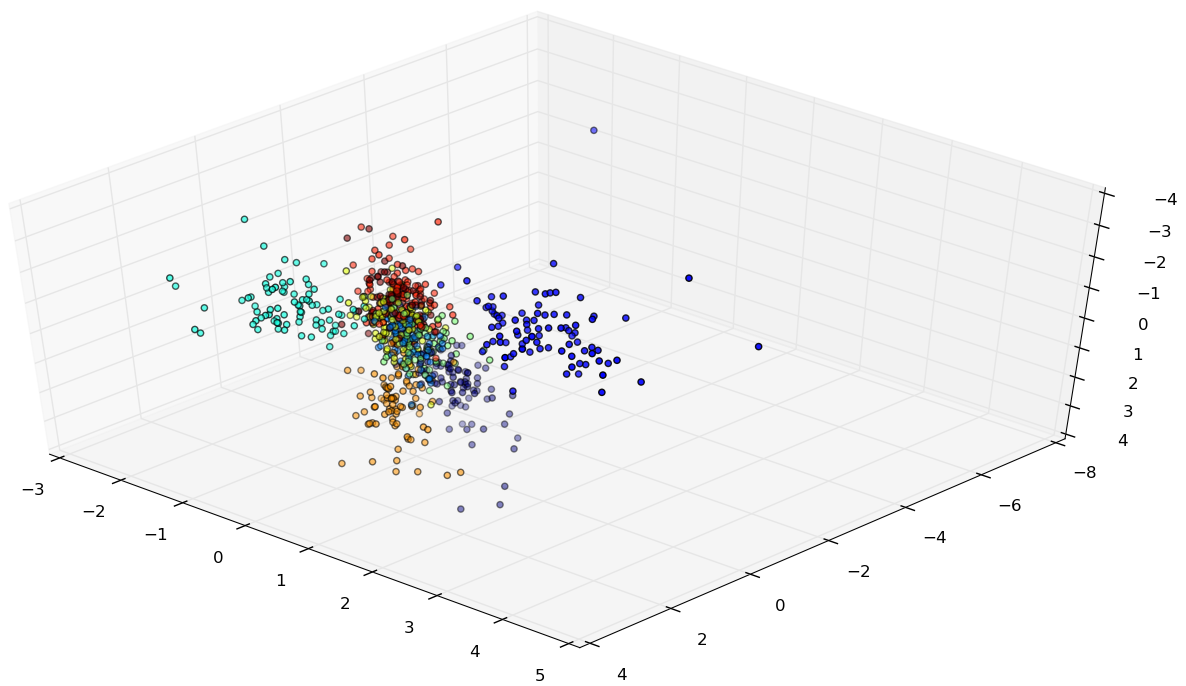
\includegraphics[width=1\linewidth, scale=1]{../img/ej1/oja/oja_3salida_200ep_train_4.png}
  \caption{Oja - 3 dimensiones - 200 épocas}
  \label{fig:sub4}
\end{subfigure}
\end{figure}

En los datos de entrenamiento se observa que con 200 épocas se empiezan a notar más visiblemente
los clusters de datos. Se observa una leve mejora en la clasificación con respecto a la versión de 100 épocas.

Podemos ver de todas formas que algunas de las categorías se encuentran mezcladas entre sí mientras otras están más claramente divididas.

A continuación los datos de validation.

\begin{figure}[!htbp]
\centering
\begin{subfigure}{.5\textwidth}
  \centering
  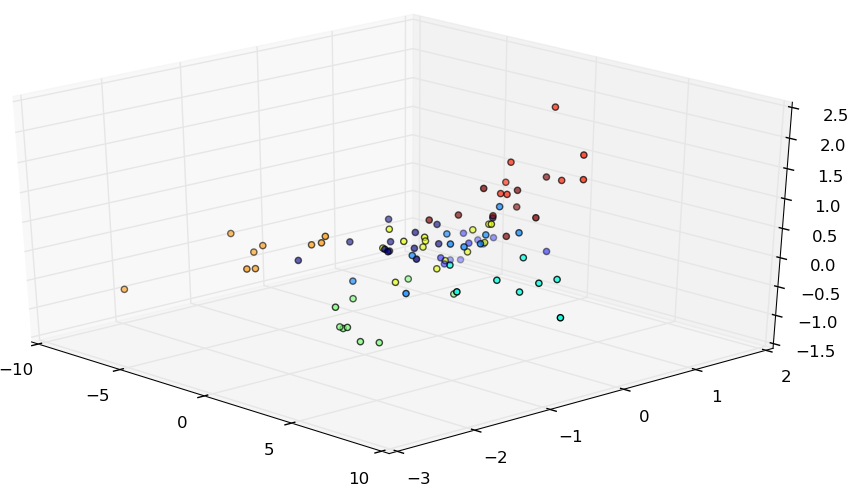
\includegraphics[width=1\linewidth, scale=1]{../img/ej1/oja/oja_3salida_200ep_validation.png}
  \caption{Oja - 3 dimensiones - 200 épocas}
  \label{fig:sub1}
\end{subfigure}%
\begin{subfigure}{.5\textwidth}
  \centering
  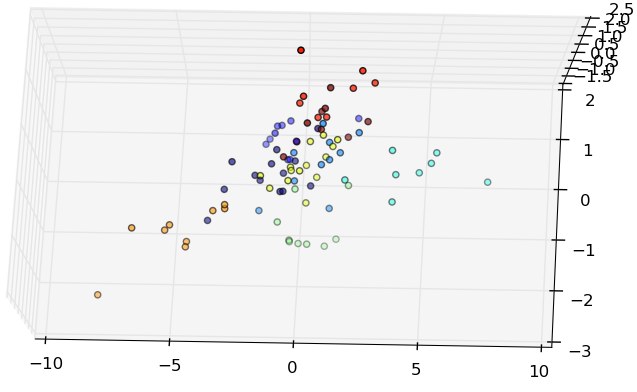
\includegraphics[width=1\linewidth, scale=1]{../img/ej1/oja/oja_3salida_200ep_validation_3.png}
  \caption{Oja - 3 dimensiones - 200 épocas}
  \label{fig:sub2}
\end{subfigure}
\end{figure}

\begin{figure}[h]
  \begin{center}
    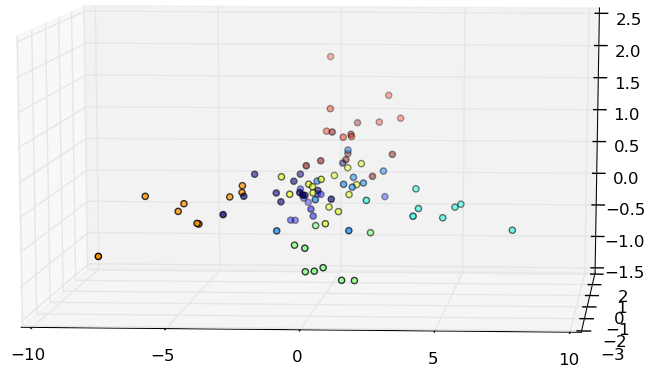
\includegraphics[scale=0.65]{../img/ej1/oja/oja_3salida_200ep_validation_2.png}
  \caption{Oja - 3 dimensiones - 200 épocas - Datos Validación}
  \end{center}
\end{figure}

En esta segunda tanda de gráficos se observa una mejora leve también para los datos de validación. Podemos ver que la mayoría de las marcas del mismo color están aproximadamente cercanas entre sí.

\subsubsection{Regla de Sanger - variando número de épocas}
Repetimos en este caso el experimento anterior utilizando ahora la regla de Sanger. Intentaremos comprobar si con esta nueva regla de aprendizaje
se obtienen mejores resultados variando el número de épocas.

En primer lugar, resultados con 100 épocas:

\newpage

\begin{figure}[!htbp]
\centering
\begin{subfigure}{.5\textwidth}
  \centering
  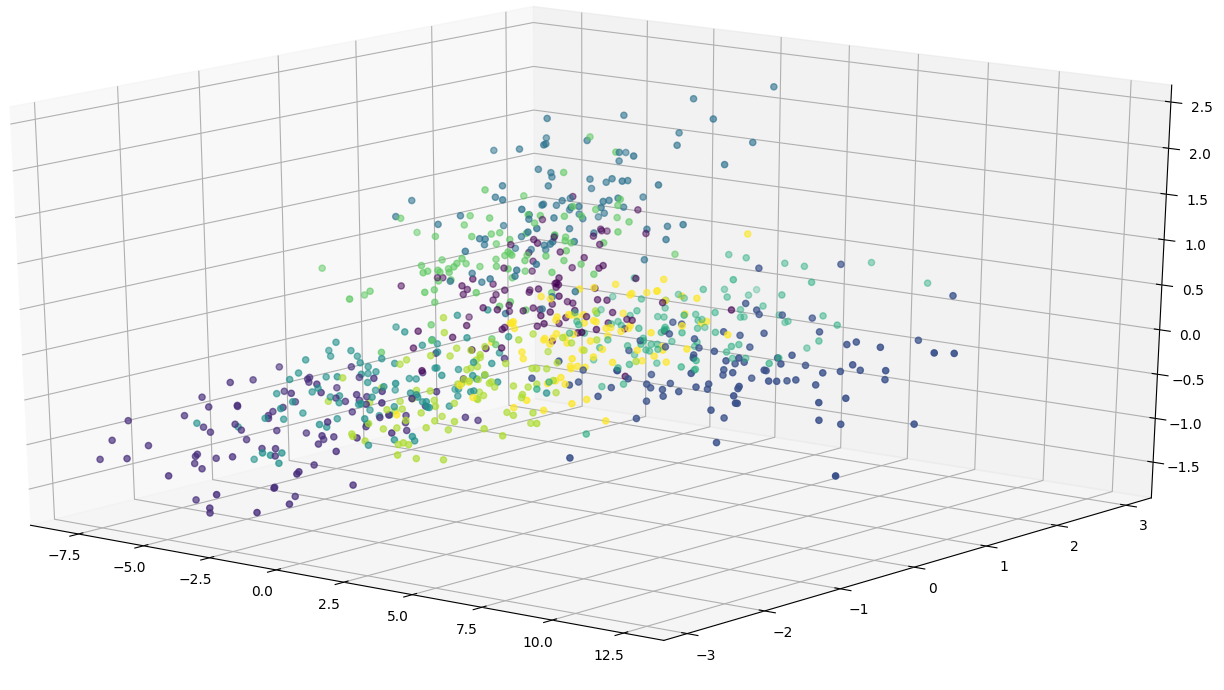
\includegraphics[width=1\linewidth, scale=1]{../img/ej1/sanger/sanger_3salida_100ep_train.png}
  \caption{Sanger - 3 dimensiones - 100 épocas}
  \label{fig:sub1}
\end{subfigure}%
\begin{subfigure}{.5\textwidth}
  \centering
  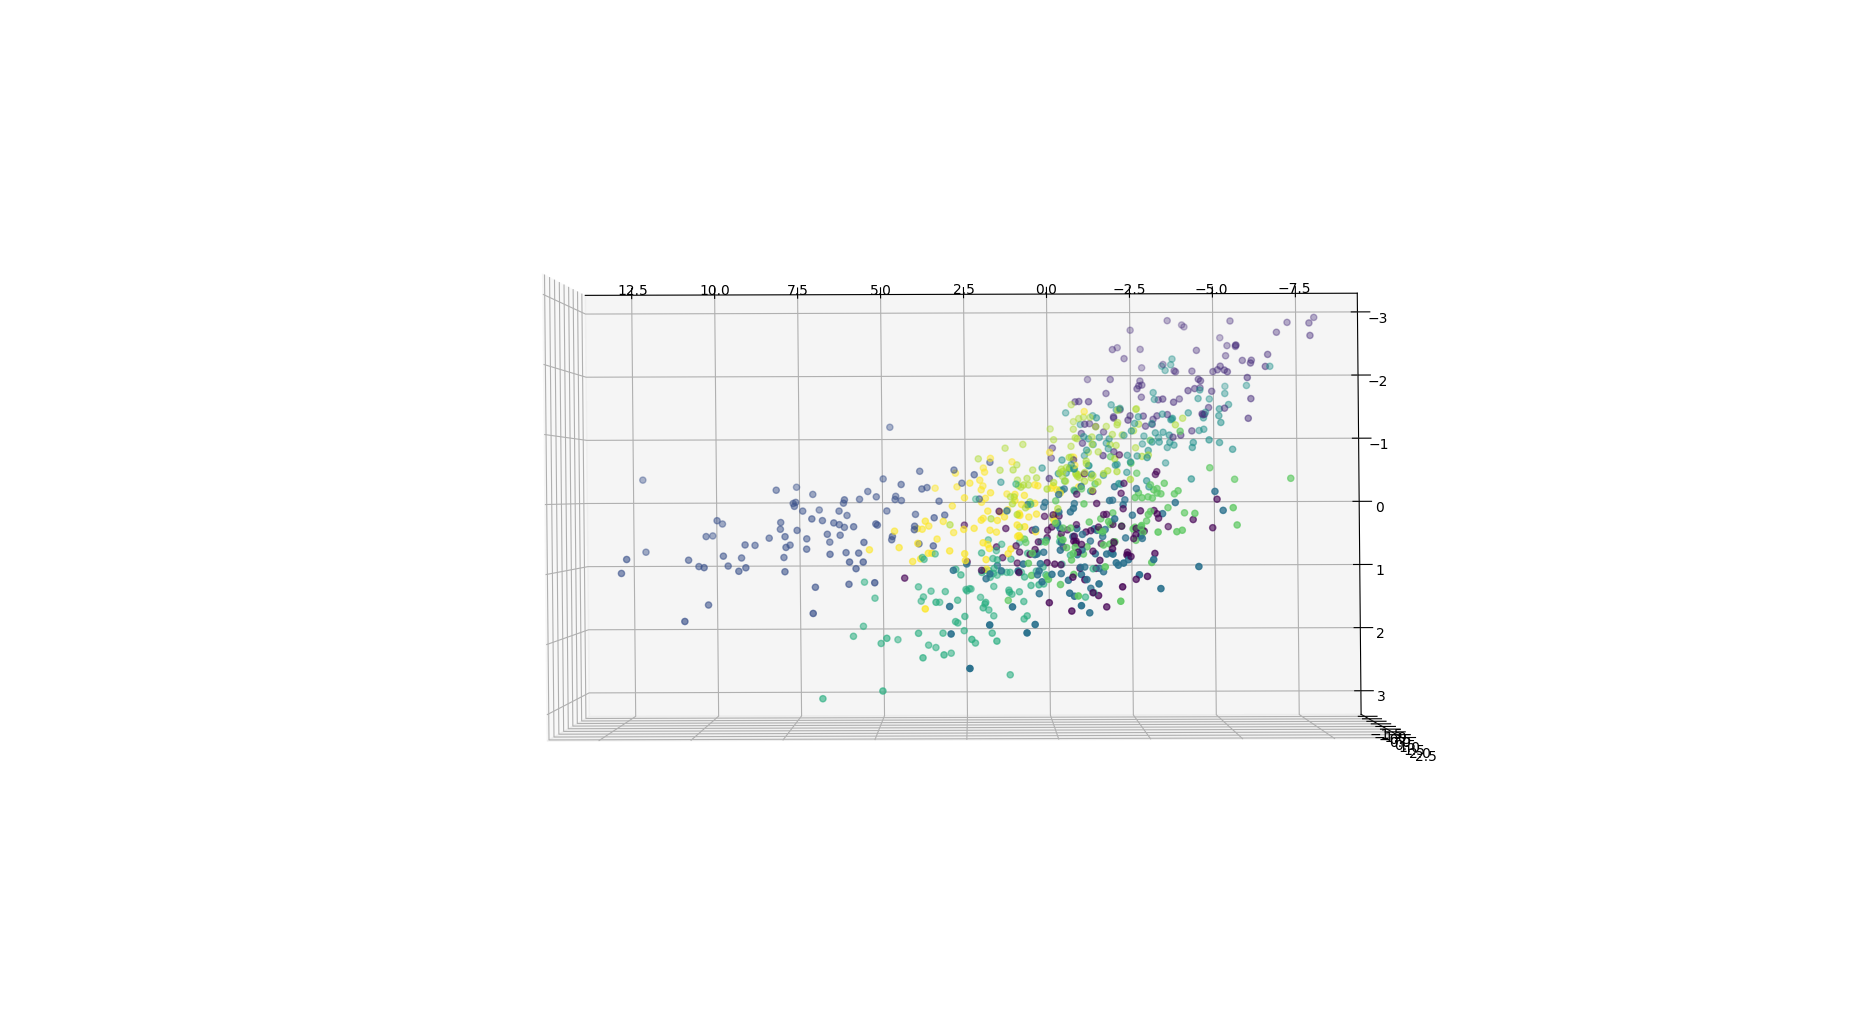
\includegraphics[width=1\linewidth, scale=1]{../img/ej1/sanger/sanger_3salida_100ep_train_3.png}
  \caption{Sanger - 3 dimensiones - 100 épocas}
  \label{fig:sub2}
\end{subfigure}
\end{figure}

\begin{figure}[h]
  \begin{center}
    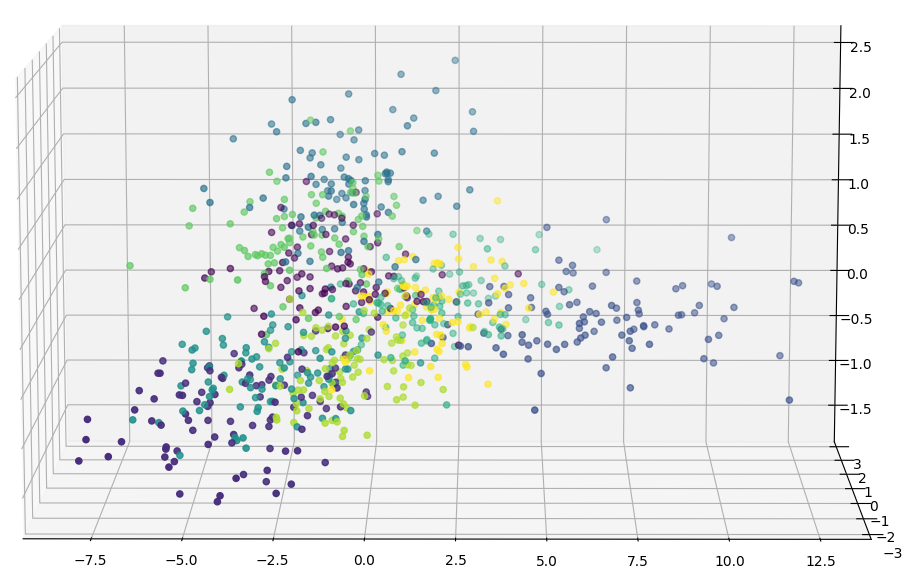
\includegraphics[scale=0.45]{../img/ej1/sanger/sanger_3salida_100ep_train_2.png}
  \caption{Sanger - 3 dimensiones - 100 épocas - Datos Entrenamiento}
  \end{center}
\end{figure}

Éstos son los resultados de las ejecuciones utilizando regla de Sanger, con 100 épocas. Notamos un gran nivel de dispersión y 
solapamiento entre las categorías. No tienen la calidad que esperábamos.

Luego de esta etapa de entrenamiento, procesamos los datos de validación. No obtuvimos buenos resultados, las marcas están 
medianamente agrupadas pero con alto nivel de disgregación.

\begin{figure}[!htbp]
\centering
\begin{subfigure}{.5\textwidth}
  \centering
  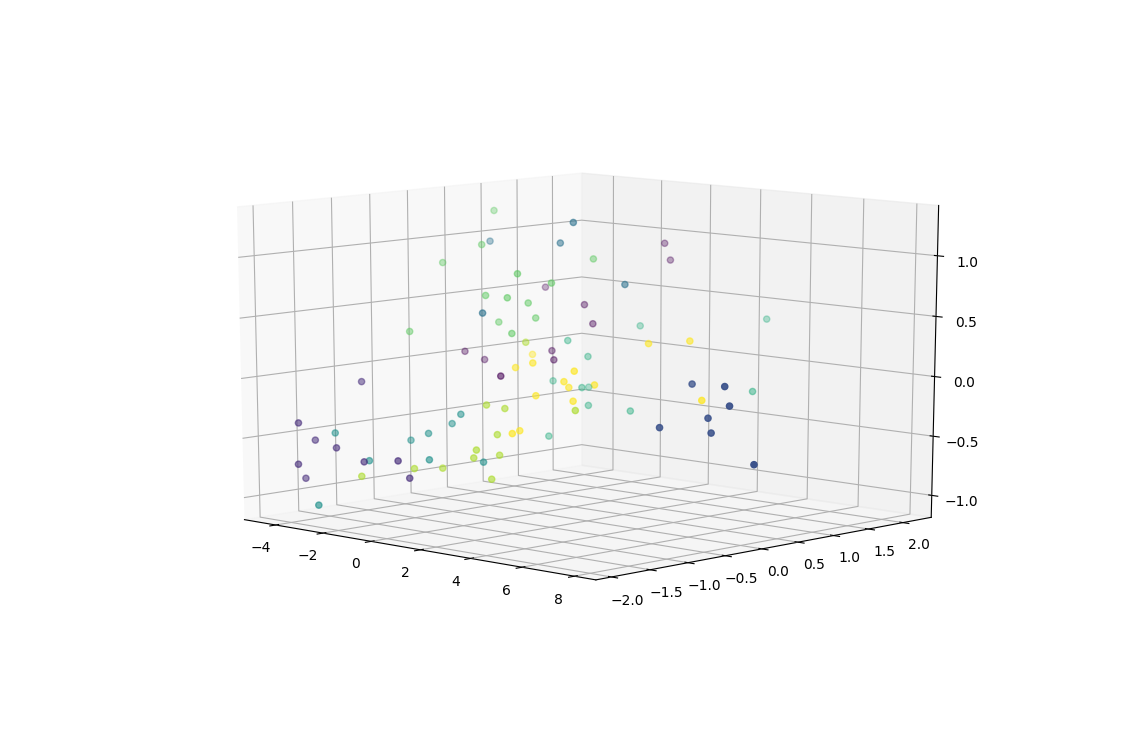
\includegraphics[width=1\linewidth, scale=1]{../img/ej1/sanger/sanger_3salida_100ep_validation.png}
  \caption{Sanger - 3 dimensiones - 100 épocas}
  \label{fig:sub1}
\end{subfigure}%
\begin{subfigure}{.5\textwidth}
  \centering
  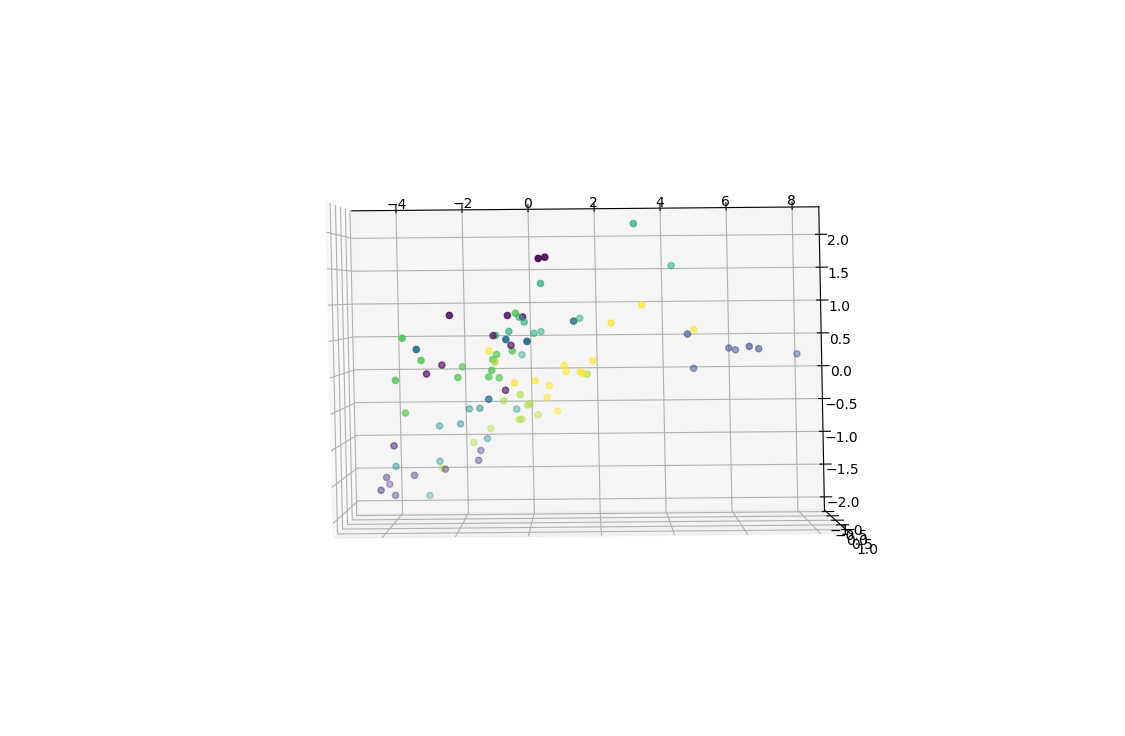
\includegraphics[width=1\linewidth, scale=1]{../img/ej1/sanger/sanger_3salida_100ep_validation_3.png}
  \caption{Sanger - 3 dimensiones - 100 épocas}
  \label{fig:sub2}
\end{subfigure}
\end{figure}

\begin{figure}[h]
  \begin{center}
    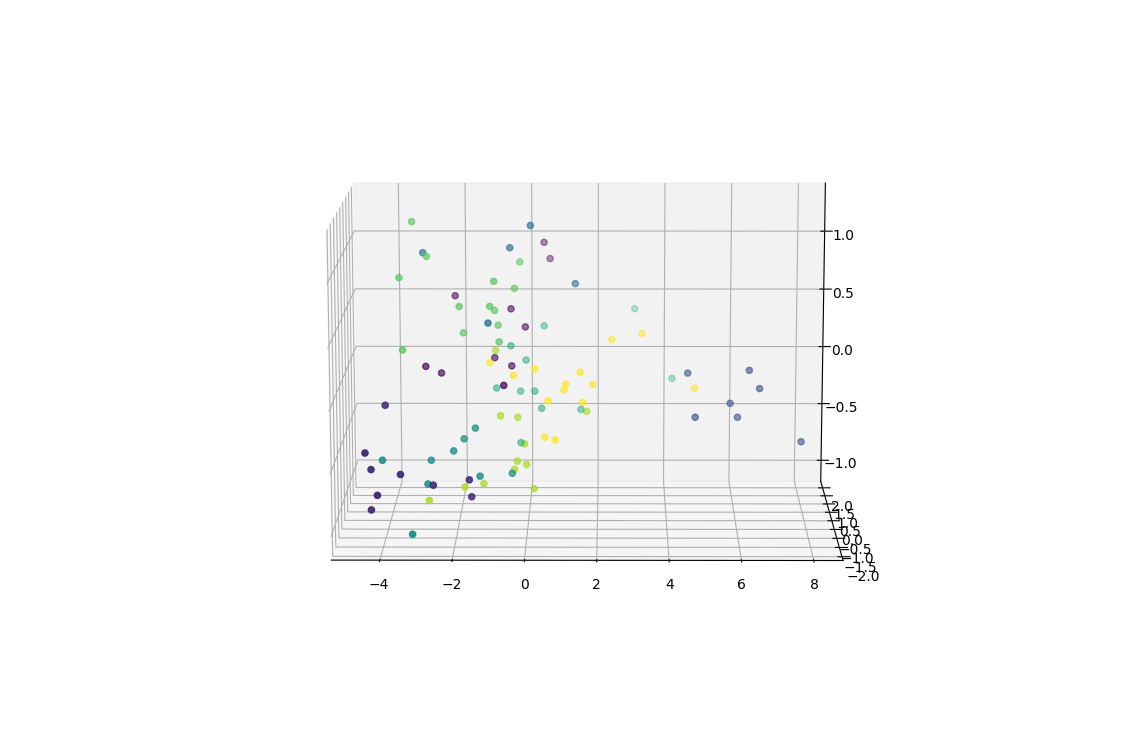
\includegraphics[scale=0.65]{../img/ej1/sanger/sanger_3salida_100ep_validation_2.png}
  \caption{Sanger - 3 dimensiones - 100 épocas - Datos Validación}
  \end{center}
\end{figure}

\newpage

Para los datos de validación vemos, que al igual que en Oja, los resultados con solo 100 épocas no son los mejores.

Observemos a continuación las mismas ejecuciones, pero subiendo el número de épocas a 200:

\begin{figure}[h]
  \begin{center}
    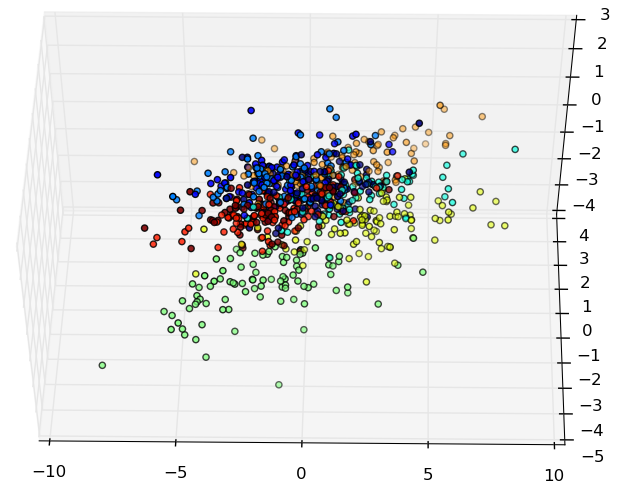
\includegraphics[scale=0.75]{../img/ej1/sanger/sanger_3salida_200ep_train_2.png}
  \caption{Sanger - 3 dimensiones - 200 épocas - Datos Validación}
  \end{center}
\end{figure}

\newpage

\begin{figure}[!htbp]
\centering
\begin{subfigure}{.5\textwidth}
  \centering
  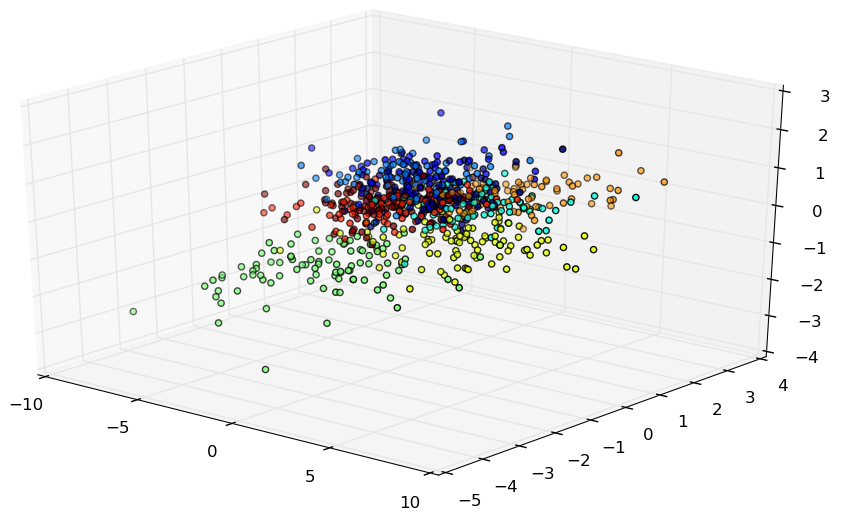
\includegraphics[width=1\linewidth, scale=1]{../img/ej1/sanger/sanger_3salida_200ep_train.png}
  \caption{Sanger - 3 dimensiones - 200 épocas}
  \label{fig:sub1}
\end{subfigure}%
\begin{subfigure}{.5\textwidth}
  \centering
  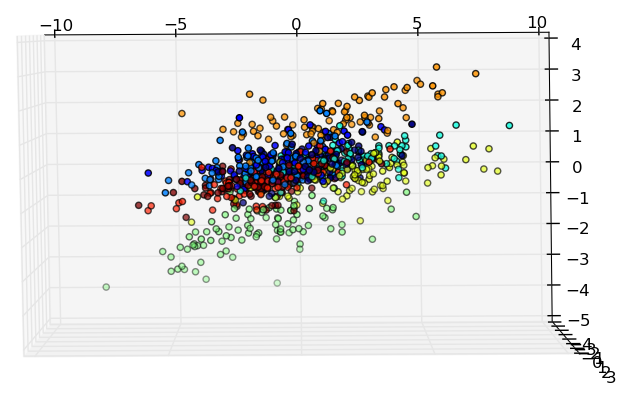
\includegraphics[width=1\linewidth, scale=1]{../img/ej1/sanger/sanger_3salida_200ep_train_3.png}
  \caption{Sanger - 3 dimensiones - 200 épocas}
  \label{fig:sub2}
\end{subfigure}
\end{figure}

En los datos de entrenamiento observamos que con 200 épocas los clusters de datos se encuentran un poco más definidos. 
Se observa una notable mejora en la clasificación con respecto a la versión anterior de 100 épocas.

Podemos ver de todas formas que algunas de las categorías presentan alto nivel de solapamiento.

A continuación los datos de validation.

\begin{figure}[!htbp]
\centering
\begin{subfigure}{.5\textwidth}
  \centering
  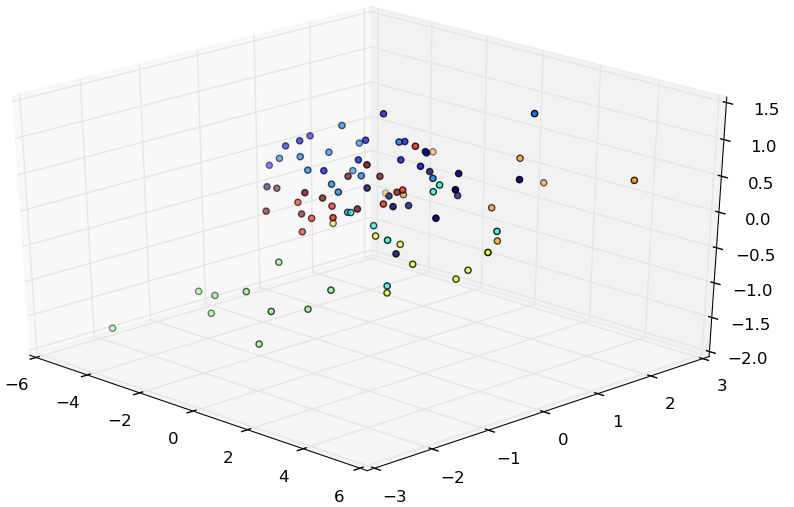
\includegraphics[width=1\linewidth, scale=1]{../img/ej1/sanger/sanger_3salida_200ep_validation.png}
  \caption{Sanger - 3 dimensiones - 200 épocas}
  \label{fig:sub1}
\end{subfigure}%
\begin{subfigure}{.5\textwidth}
  \centering
  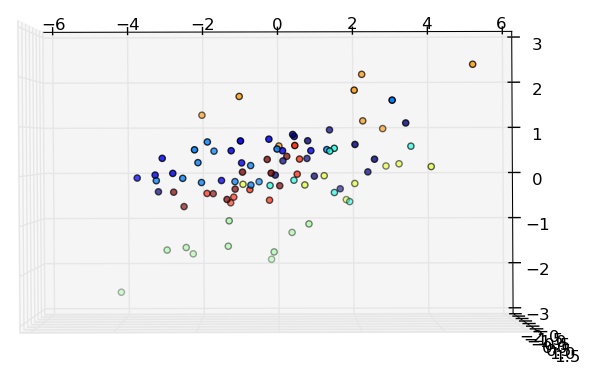
\includegraphics[width=1\linewidth, scale=1]{../img/ej1/sanger/sanger_3salida_200ep_validation_3.png}
  \caption{Sanger - 3 dimensiones - 200 épocas}
  \label{fig:sub2}
\end{subfigure}
\end{figure}

\begin{figure}[h]
  \begin{center}
    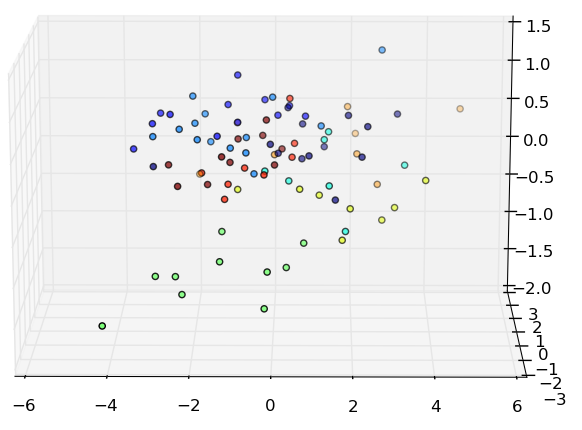
\includegraphics[scale=0.4]{../img/ej1/sanger/sanger_3salida_200ep_validation_2.png}
  \caption{Sanger - 3 dimensiones - 200 épocas - Datos Validación}
  \end{center}
\end{figure}

En esta segunda tanda de gráficos se observa una mejora leve también para los datos de validación. Podemos ver que la mayoría de las marcas del mismo color están aproximadamente cercanas entre sí.

Debido a la lenta performance de las pruebas con la red, continuar aumentando la cantidad de épocas se volvió inviable. De todas formas hicimos una prueba preliminar con 500 épocas para explorar la posibilidad de obtener mejores resultados. Éstos no fueron mejores que los presentados aquí con 200, por lo tanto no continuamos dicho experimento y nos quedamos con las 200.
\newpage
\subsubsection{Regla de Oja - Variando número de dimensiones}

Dados los resultados obtenidos, intentamos buscar una forma de mejorar la precisión de la clasificación. Por sugerencia docente, decidimos intentar aumentar la dimensionalidad de la salida. En lugar de reducir a 3 dimensiones como pide el enunciado, subimos la cantidad a 9 dimensiones, esperando obtener mejores resultados. \\
Teniendo en cuenta la imposibilidad de graficar y observar espacialmente los resultados con 9 valores, partimos los vectores de salida y mostramos 3 espacios tridimensionales con 3 características cada uno. El procedimiento fue tomar las primeras 3 dimensiones de cada resultado, graficarlas en 3D, luego repetir con las siguientes 3 y continuar de esta forma con las últimas.

En este experimento solo mostraremos los resultados de las corridas de entrenamiento, ya que cuentan con un volumen de datos mayor y permiten apreciar mejor la división en clusters. A continuación mostraremos los resultados que obtuvimos para ambas reglas, utilizando 9 dimensiones de salida.

Comenzamos con las primeras tres coordenadas:

\begin{figure}[!htbp]
\centering
\begin{subfigure}{.5\textwidth}
  \centering
  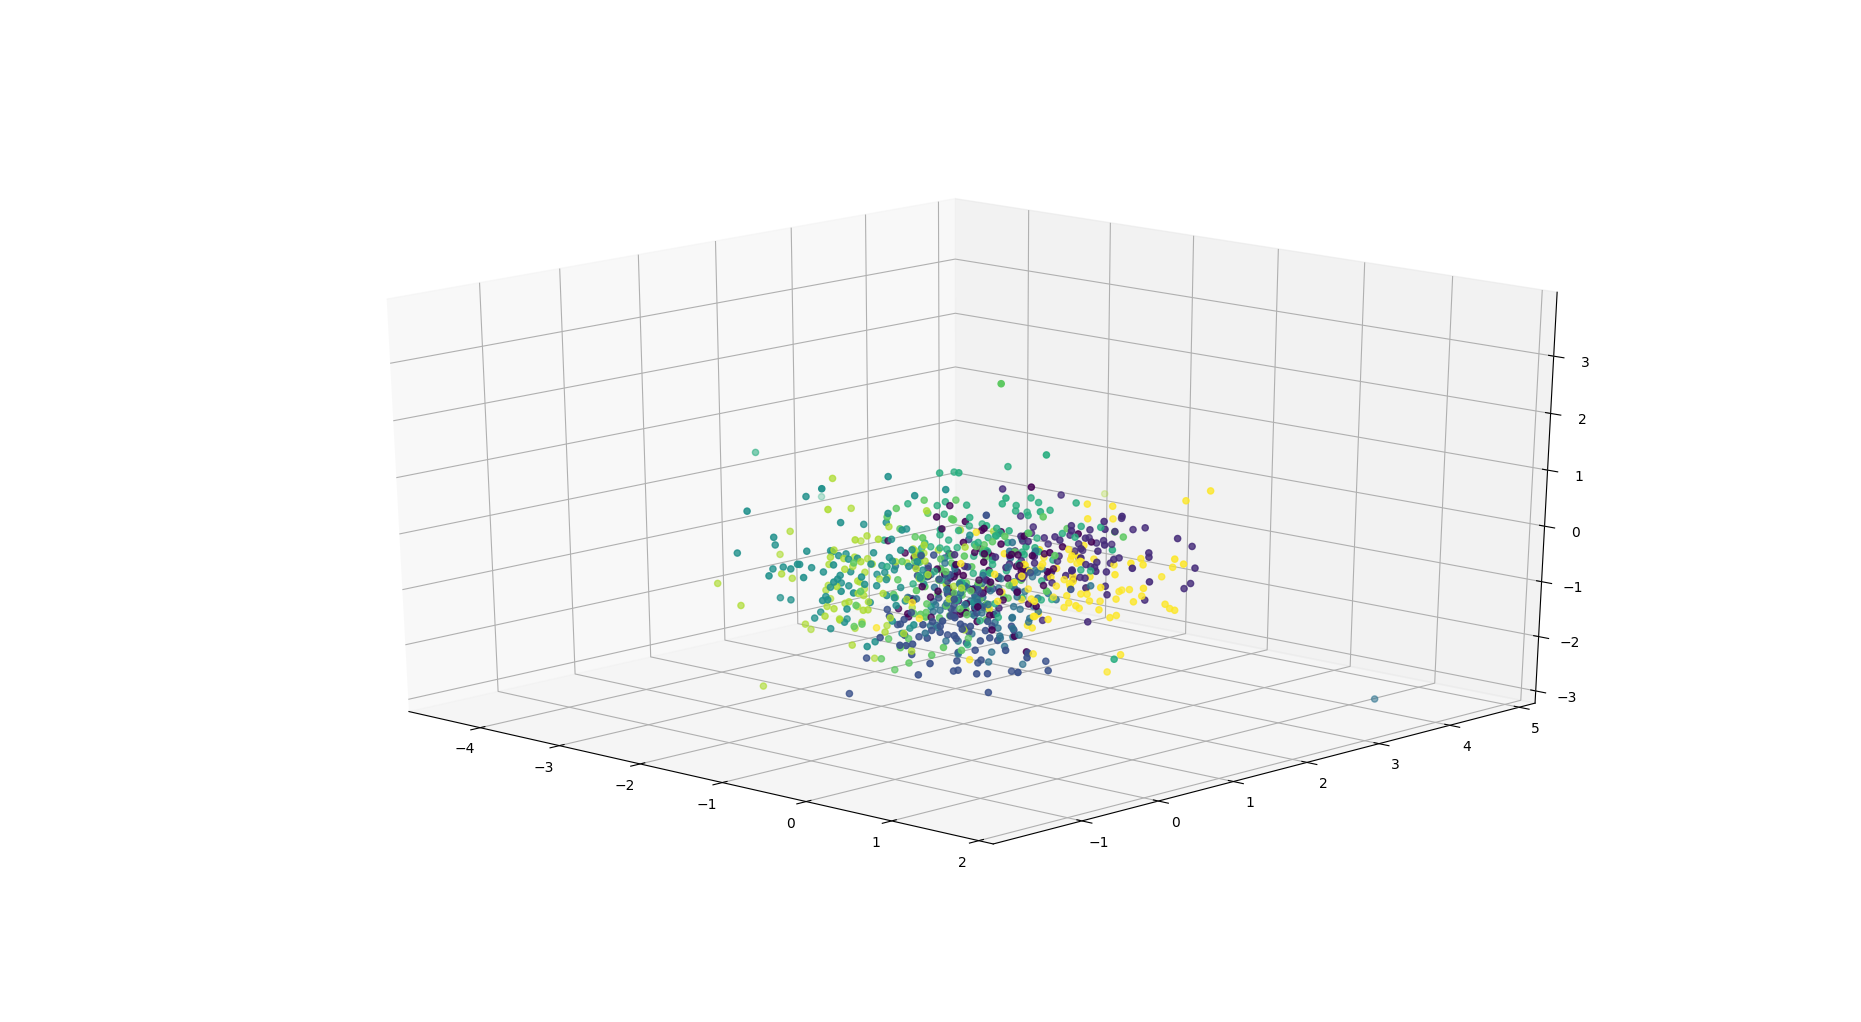
\includegraphics[width=1\linewidth, scale=1]{../img/ej1/oja_corrida_200_9/oja_9salida_200ep_testing_dim123.png}
  \caption{Oja - 9 dimensiones - 200 épocas - Coordenadas 123}
  \label{fig:sub1}
\end{subfigure}%
\begin{subfigure}{.5\textwidth}
  \centering
  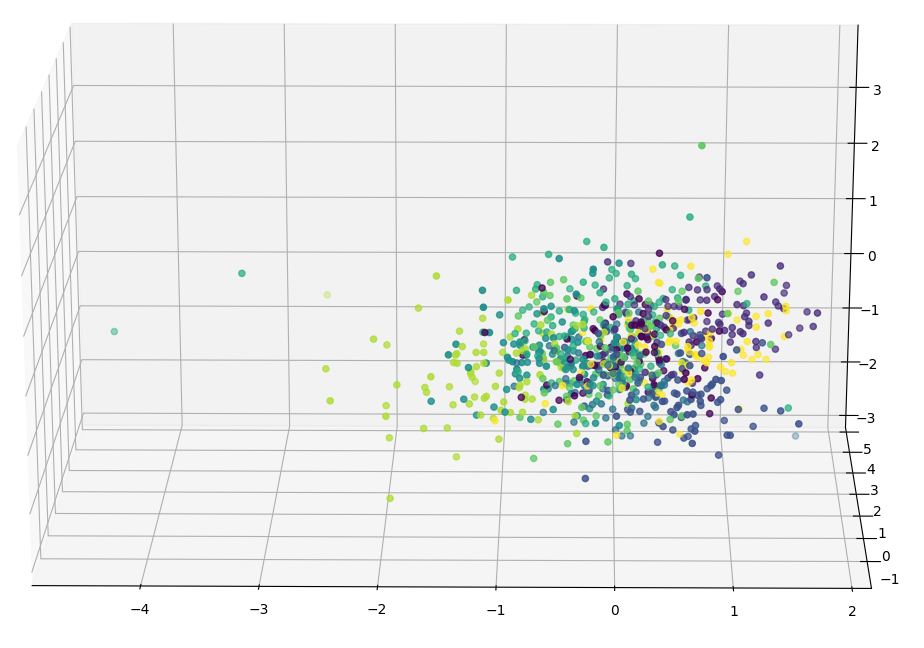
\includegraphics[width=1\linewidth, scale=1]{../img/ej1/oja_corrida_200_9/oja_9salida_200ep_testing_dim123_2.png}
  \caption{Oja - 9 dimensiones - 200 épocas - Coordenadas 123}
  \label{fig:sub2}
\end{subfigure}
\end{figure}

\begin{figure}[!htbp]
\centering
\begin{subfigure}{.5\textwidth}
  \centering
  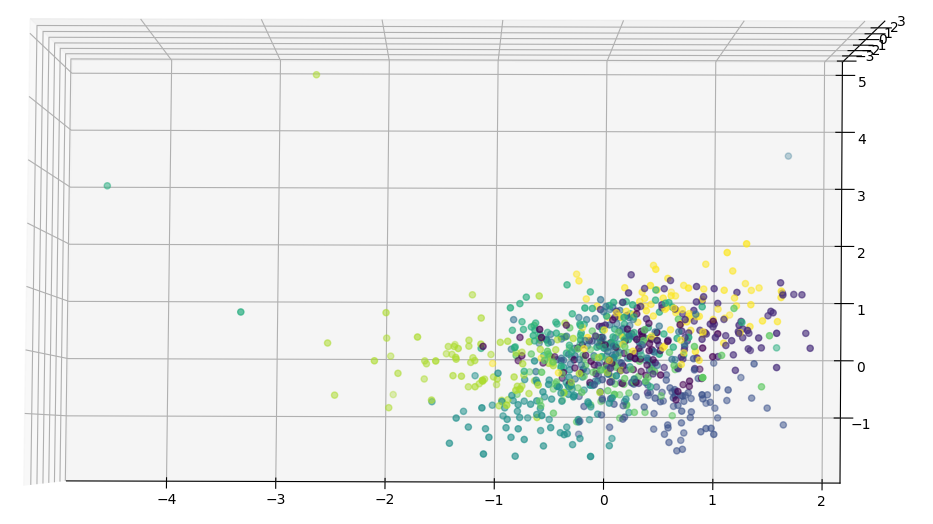
\includegraphics[width=1\linewidth, scale=1]{../img/ej1/oja_corrida_200_9/oja_9salida_200ep_testing_dim123_3.png}
  \caption{Oja - 9 dimensiones - 200 épocas - Coordenadas 123}
  \label{fig:sub1}
\end{subfigure}%
\begin{subfigure}{.5\textwidth}
  \centering
  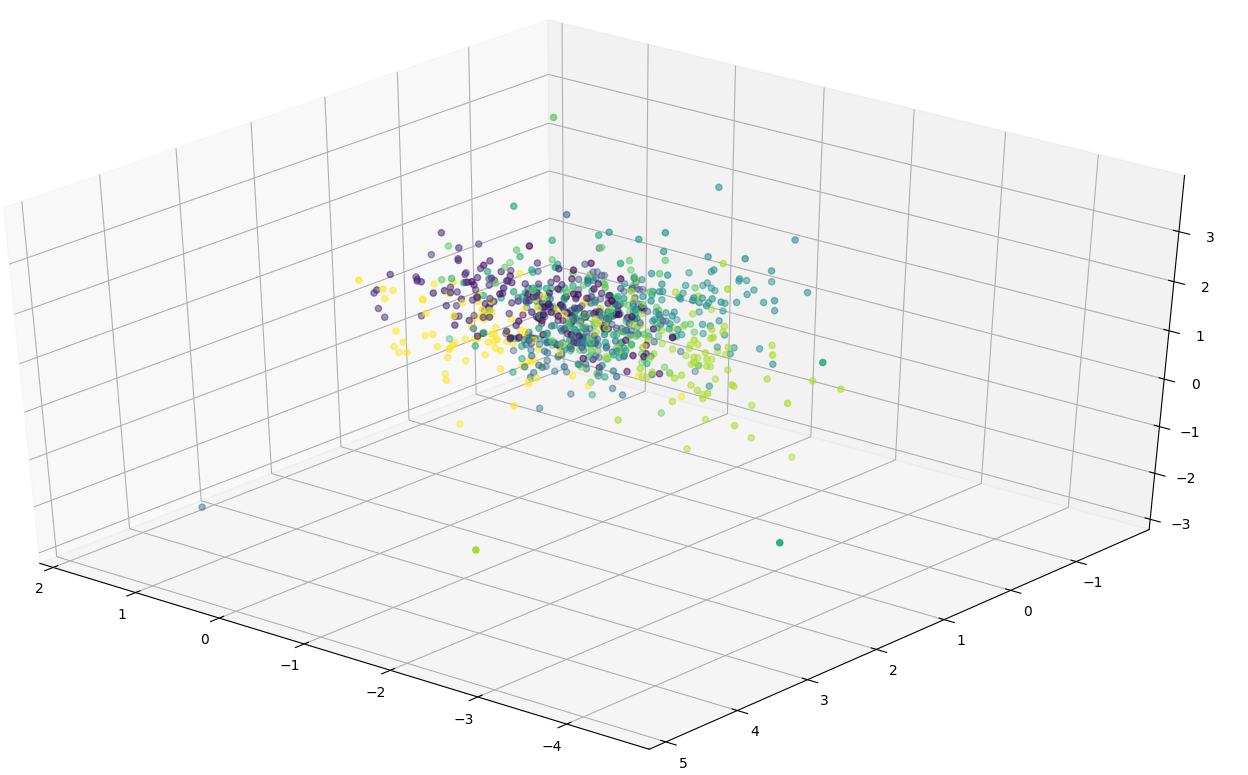
\includegraphics[width=1\linewidth, scale=1]{../img/ej1/oja_corrida_200_9/oja_9salida_200ep_testing_dim123_4.png}
  \caption{Oja - 9 dimensiones - 200 épocas - Coordenadas 123}
  \label{fig:sub2}
\end{subfigure}
\end{figure}

\newpage

En estas primeras 3 coordenadas, los clusters se encuentran muy entrelazados y mezclados, la clasificación no es clara. No se observan demasiadas mejoras
contra la versión de 3 dimensiones únicas.

Veamos las siguientes 3 coordenadas.

\begin{figure}[!htbp]
\centering
\begin{subfigure}{.5\textwidth}
  \centering
  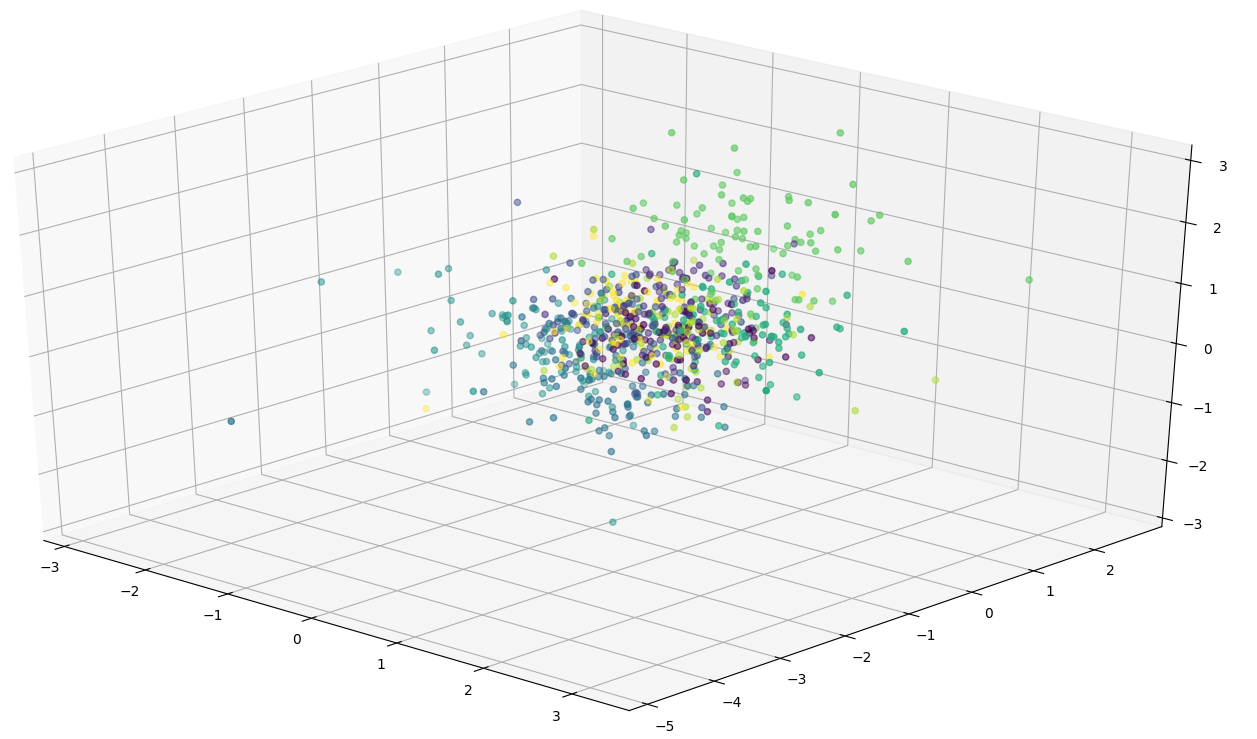
\includegraphics[width=1\linewidth, scale=1]{../img/ej1/oja_corrida_200_9/oja_9salida_200ep_testing_dim456.png}
  \caption{Oja - 9 dimensiones - 200 épocas - Coordenadas 456}
  \label{fig:sub1}
\end{subfigure}%
\begin{subfigure}{.5\textwidth}
  \centering
  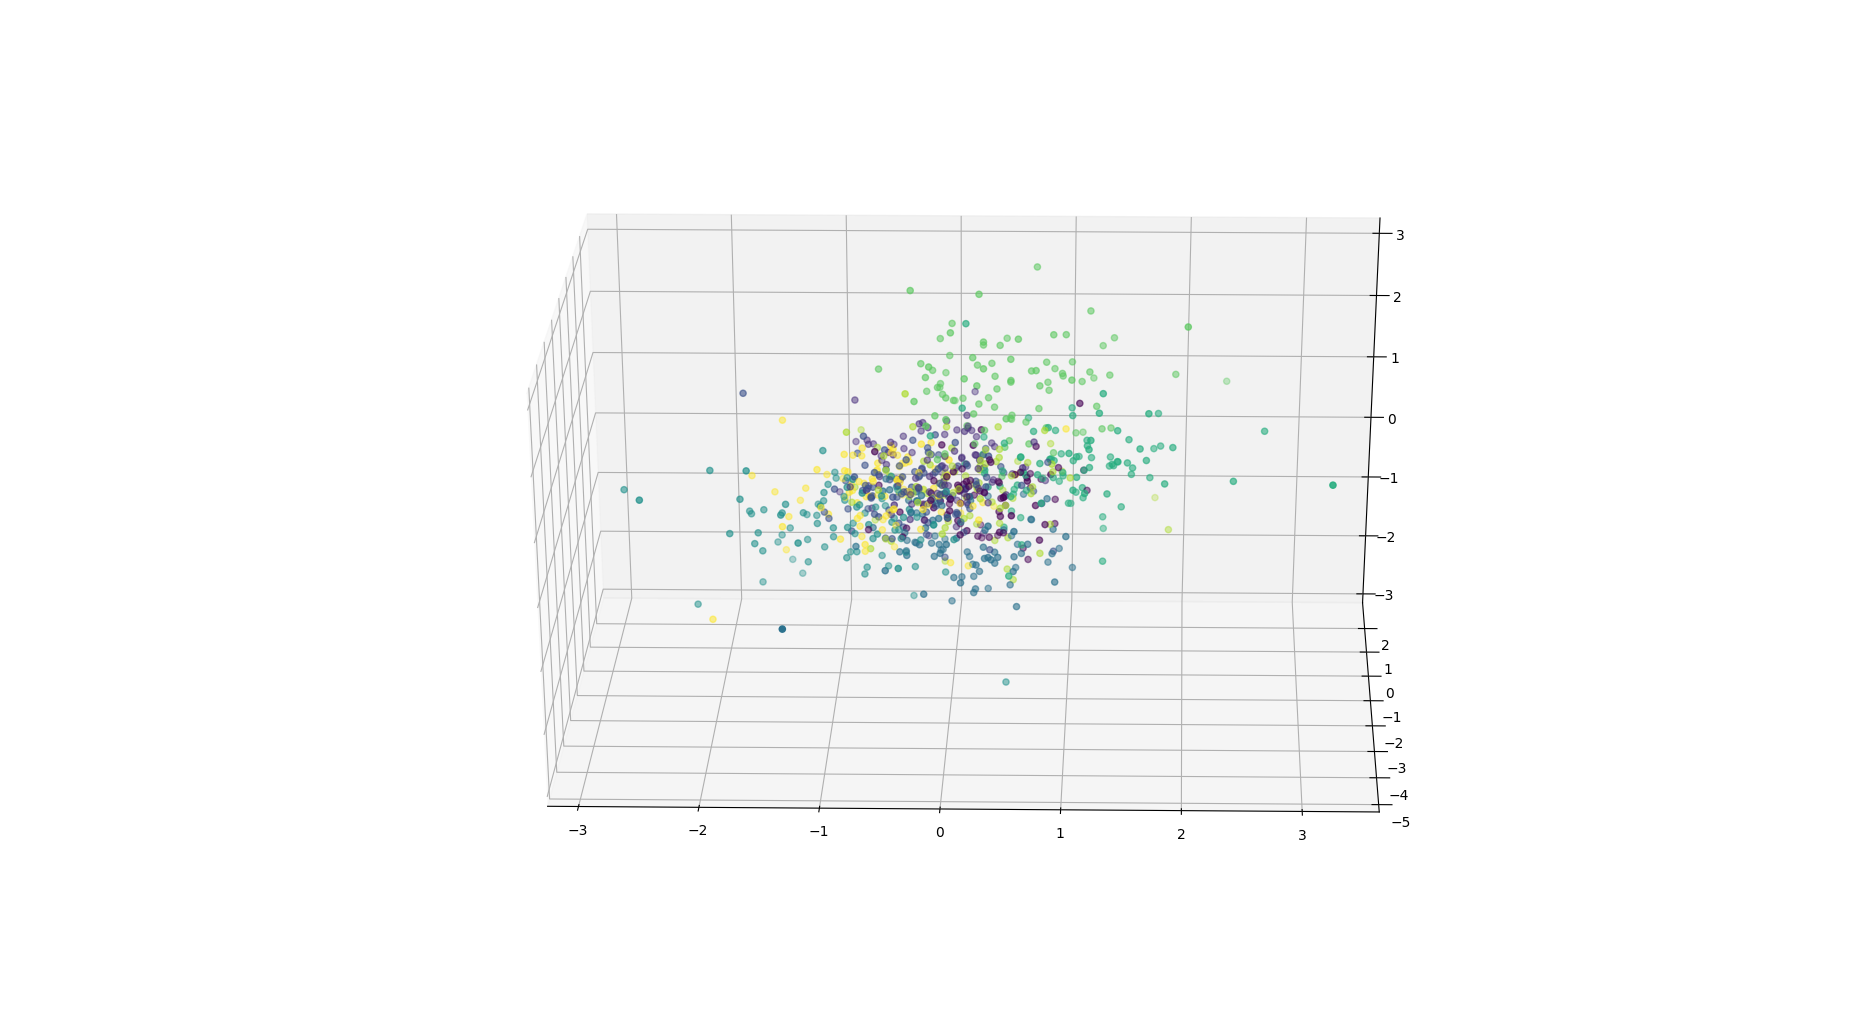
\includegraphics[width=1\linewidth, scale=1]{../img/ej1/oja_corrida_200_9/oja_9salida_200ep_testing_dim456_2.png}
  \caption{Oja - 9 dimensiones - 200 épocas - Coordenadas 456}
  \label{fig:sub2}
\end{subfigure}
\end{figure}

\begin{figure}[!htbp]
\centering
\begin{subfigure}{.5\textwidth}
  \centering
  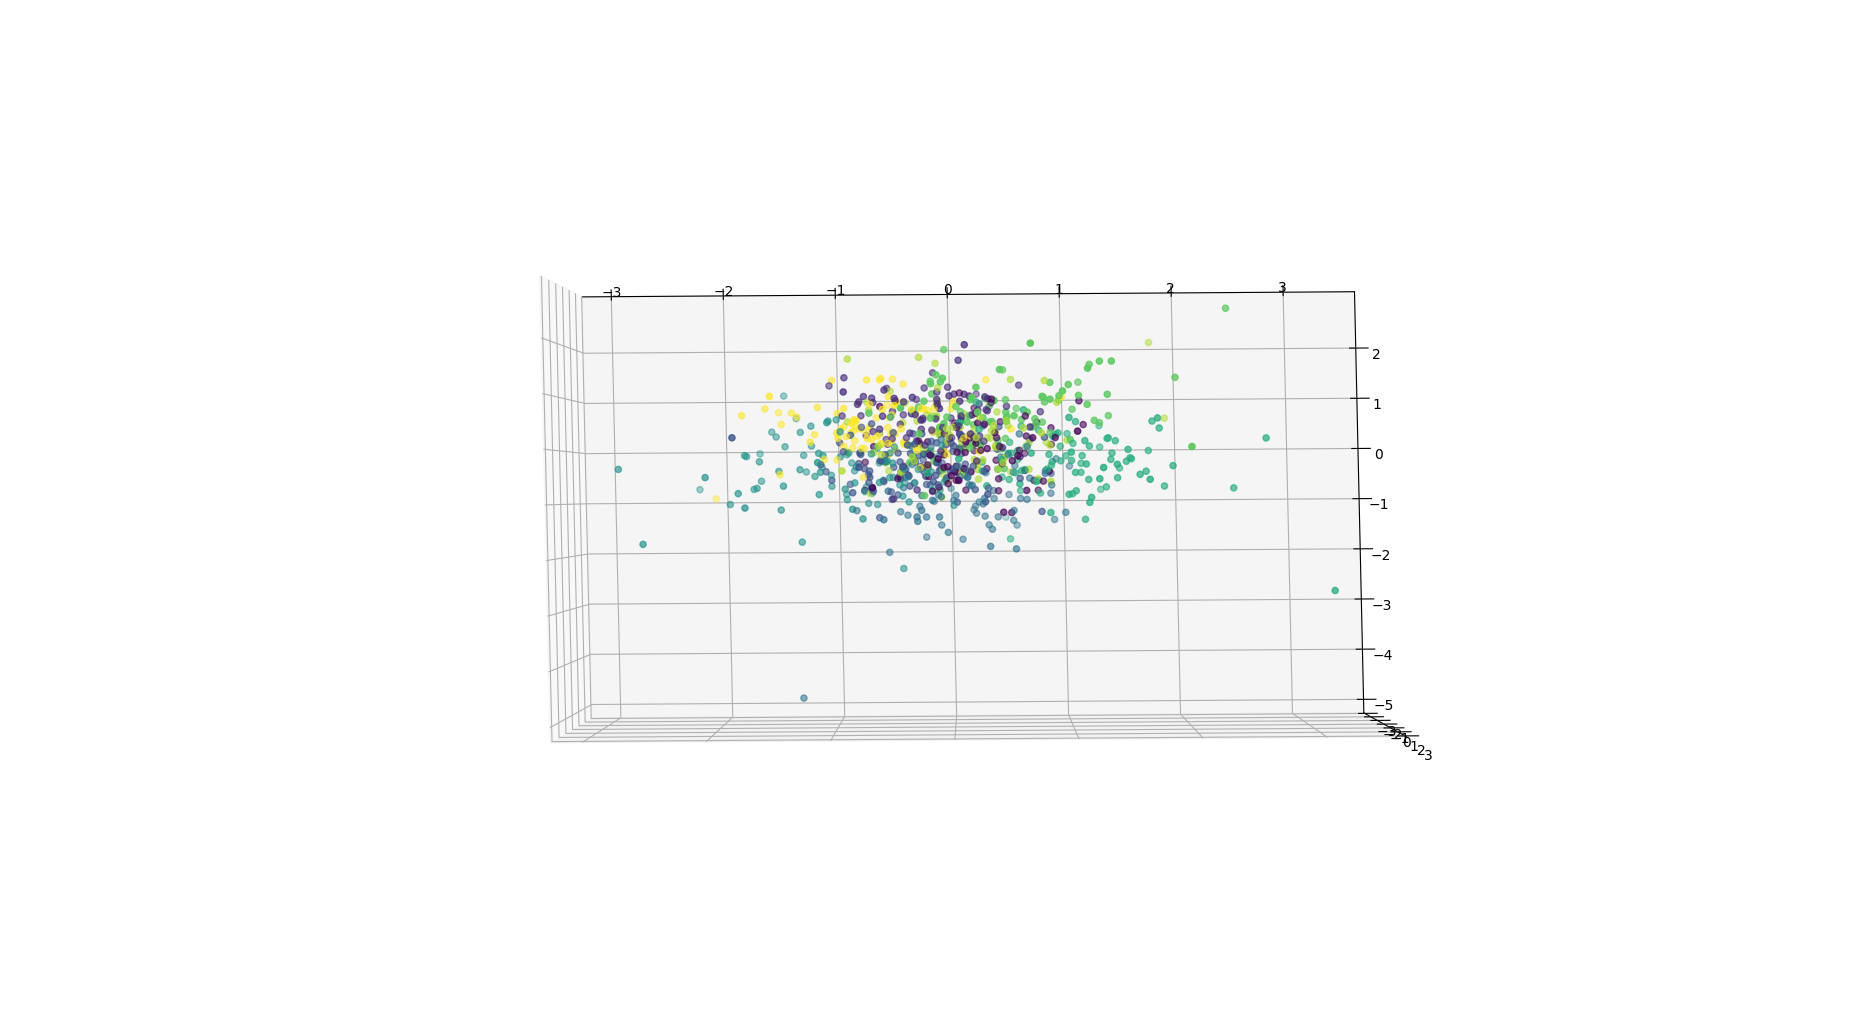
\includegraphics[width=1\linewidth, scale=1]{../img/ej1/oja_corrida_200_9/oja_9salida_200ep_testing_dim456_3.png}
  \caption{Oja - 9 dimensiones - 200 épocas - Coordenadas 456}
  \label{fig:sub1}
\end{subfigure}%
\begin{subfigure}{.5\textwidth}
  \centering
  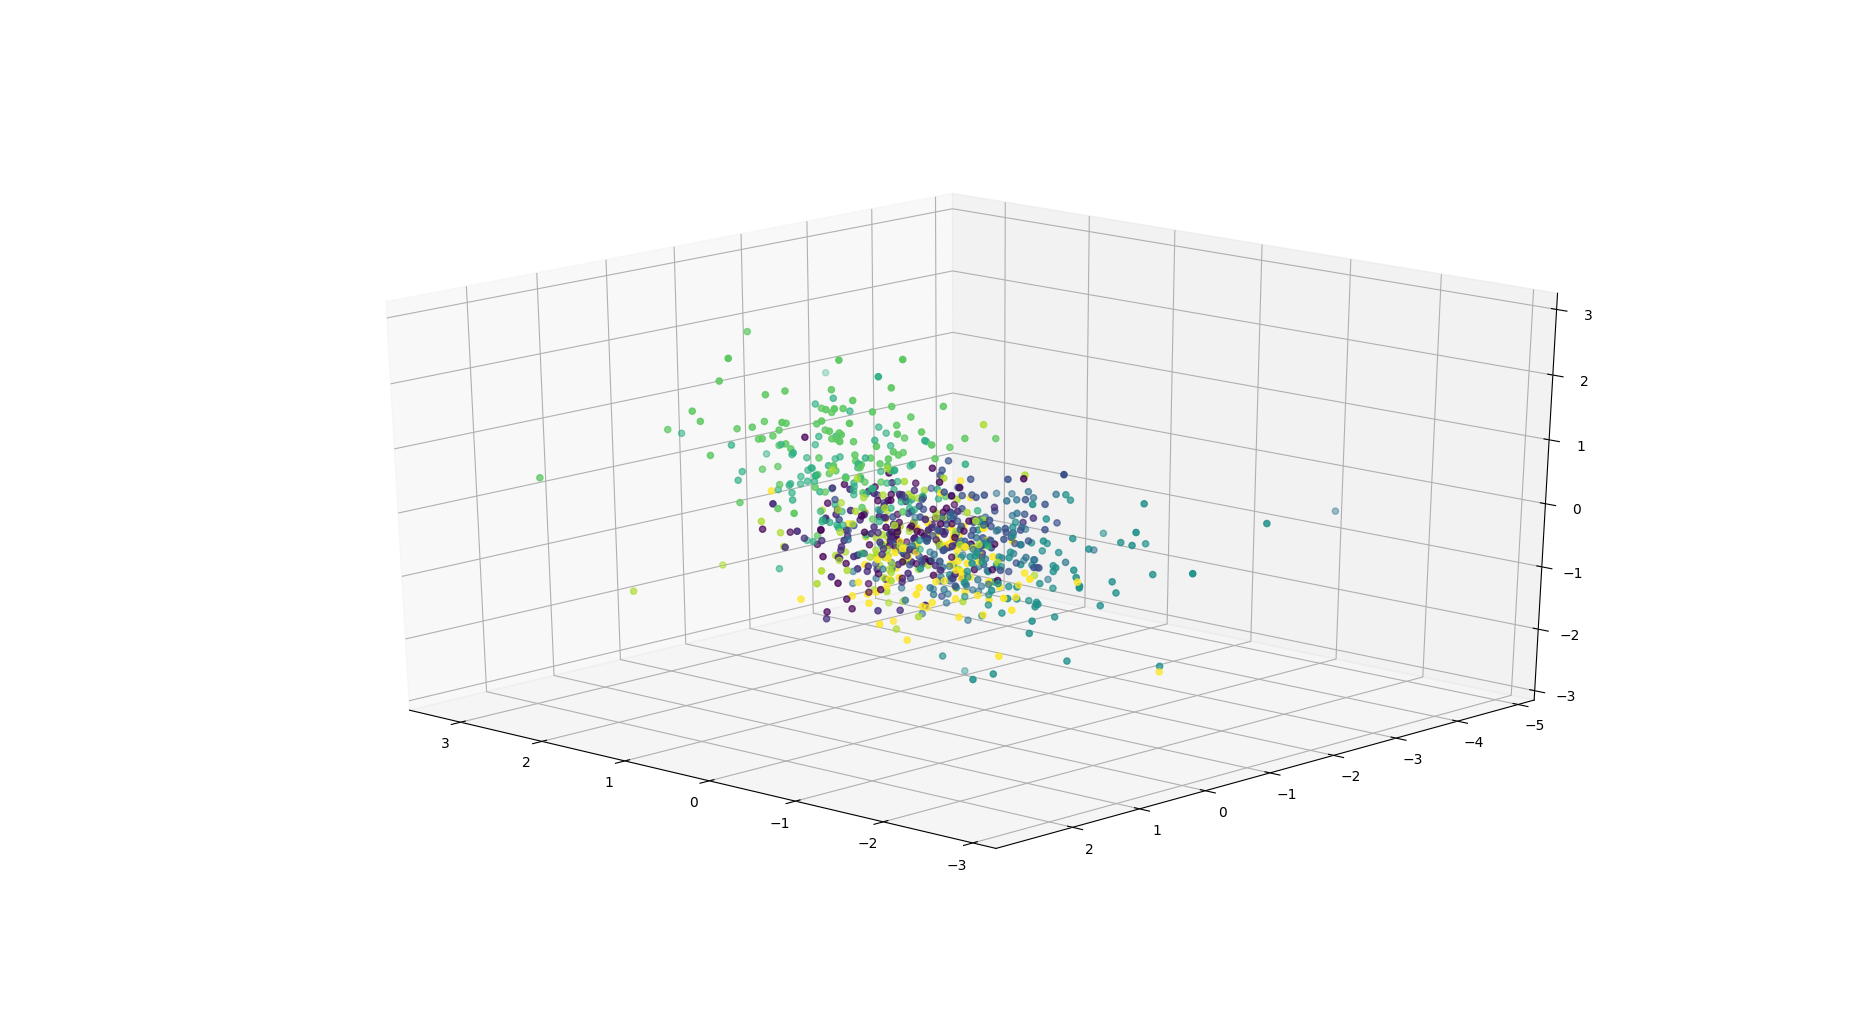
\includegraphics[width=1\linewidth, scale=1]{../img/ej1/oja_corrida_200_9/oja_9salida_200ep_testing_dim456_4.png}
  \caption{Oja - 9 dimensiones - 200 épocas - Coordenadas 456}
  \label{fig:sub2}
\end{subfigure}
\end{figure}

Para las coordenadas 456 vemos que hay una mayor expansión del espacio ocupado por los datos y se nota un grado levemente mayor de separación entre
los puntos coloreados.

Veamos las siguientes 3 coordenadas.

\begin{figure}[!htbp]
\centering
\begin{subfigure}{.5\textwidth}
  \centering
  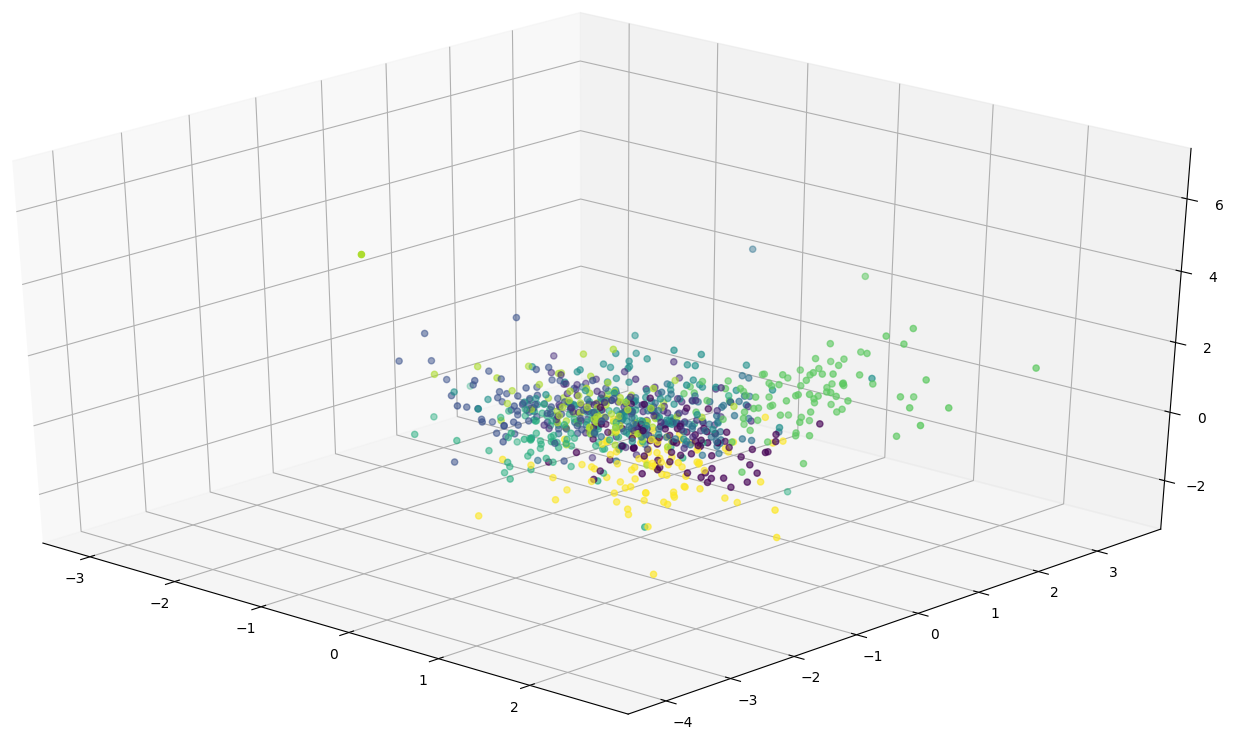
\includegraphics[width=1\linewidth, scale=1]{../img/ej1/oja_corrida_200_9/oja_9salida_200ep_testing_dim789.png}
  \caption{Oja - 9 dimensiones - 200 épocas - Coordenadas 789}
  \label{fig:sub1}
\end{subfigure}%
\begin{subfigure}{.5\textwidth}
  \centering
  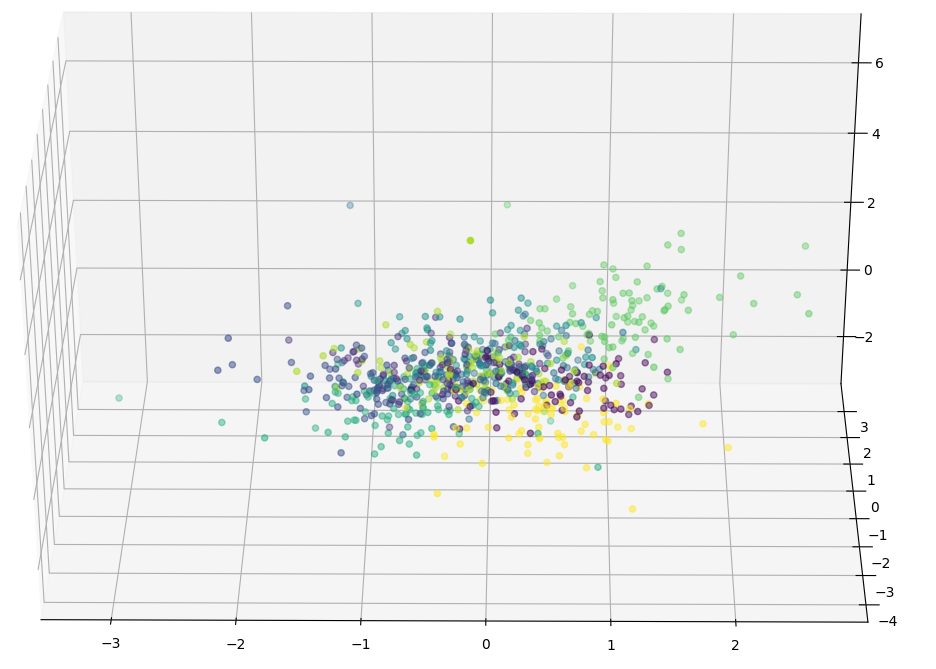
\includegraphics[width=1\linewidth, scale=1]{../img/ej1/oja_corrida_200_9/oja_9salida_200ep_testing_dim789_2.png}
  \caption{Oja - 9 dimensiones - 200 épocas - Coordenadas 789}
  \label{fig:sub2}
\end{subfigure}
\end{figure}

\begin{figure}[!htbp]
\centering
\begin{subfigure}{.5\textwidth}
  \centering
  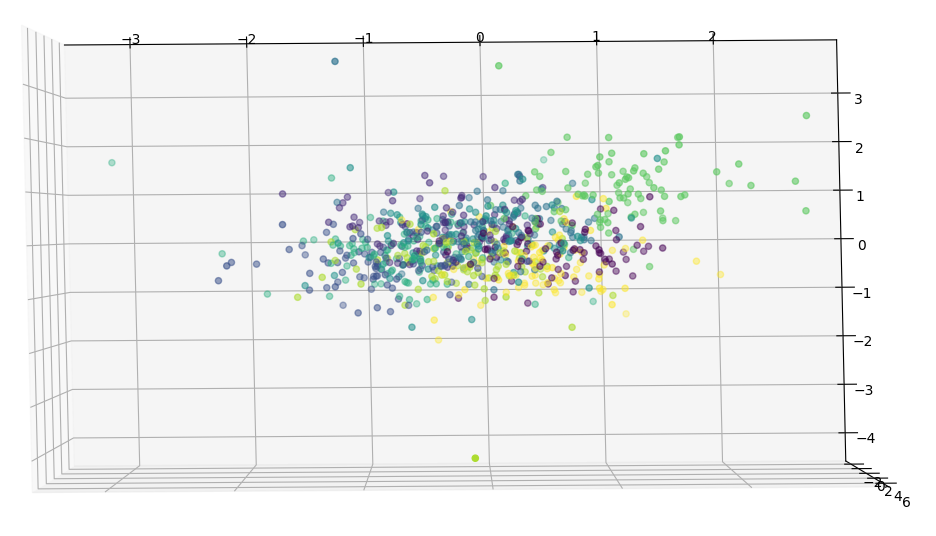
\includegraphics[width=1\linewidth, scale=1]{../img/ej1/oja_corrida_200_9/oja_9salida_200ep_testing_dim789_3.png}
  \caption{Oja - 9 dimensiones - 200 épocas - Coordenadas 789}
  \label{fig:sub1}
\end{subfigure}%
\begin{subfigure}{.5\textwidth}
  \centering
  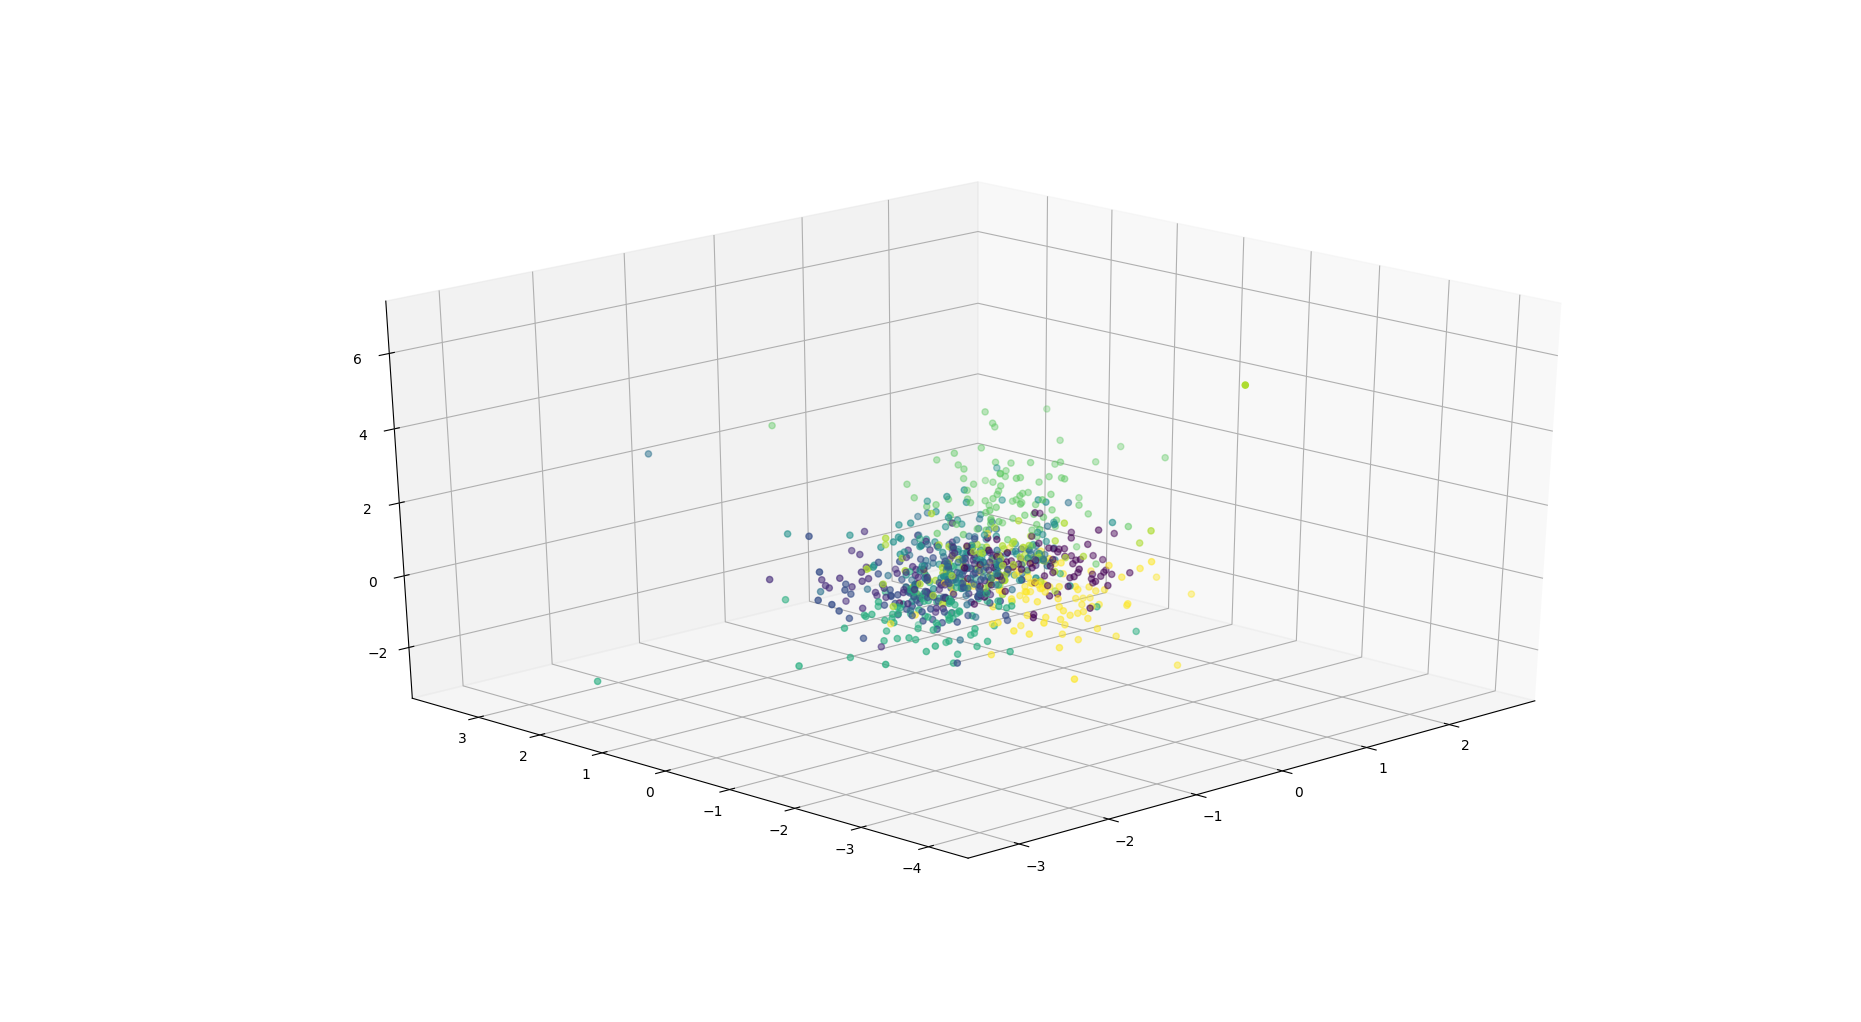
\includegraphics[width=1\linewidth, scale=1]{../img/ej1/oja_corrida_200_9/oja_9salida_200ep_testing_dim789_4.png}
  \caption{Oja - 9 dimensiones - 200 épocas - Coordenadas 789}
  \label{fig:sub2}
\end{subfigure}
\end{figure}

En las últimas coordenadas los resultados son similares a las 456. Se notan algunas zonas donde predominan cierta categoría, con bastante solapamiento en la zona central.
Los resultados no se muestran muy superiores a los obtenidos con solo 3 coordenadas totales.

Observemos las ejecuciones utilizando Regla de Sanger.

\subsubsection{Regla de Sanger - Variando número de dimensiones}

\begin{figure}[!htbp]
\centering
\begin{subfigure}{.5\textwidth}
  \centering
  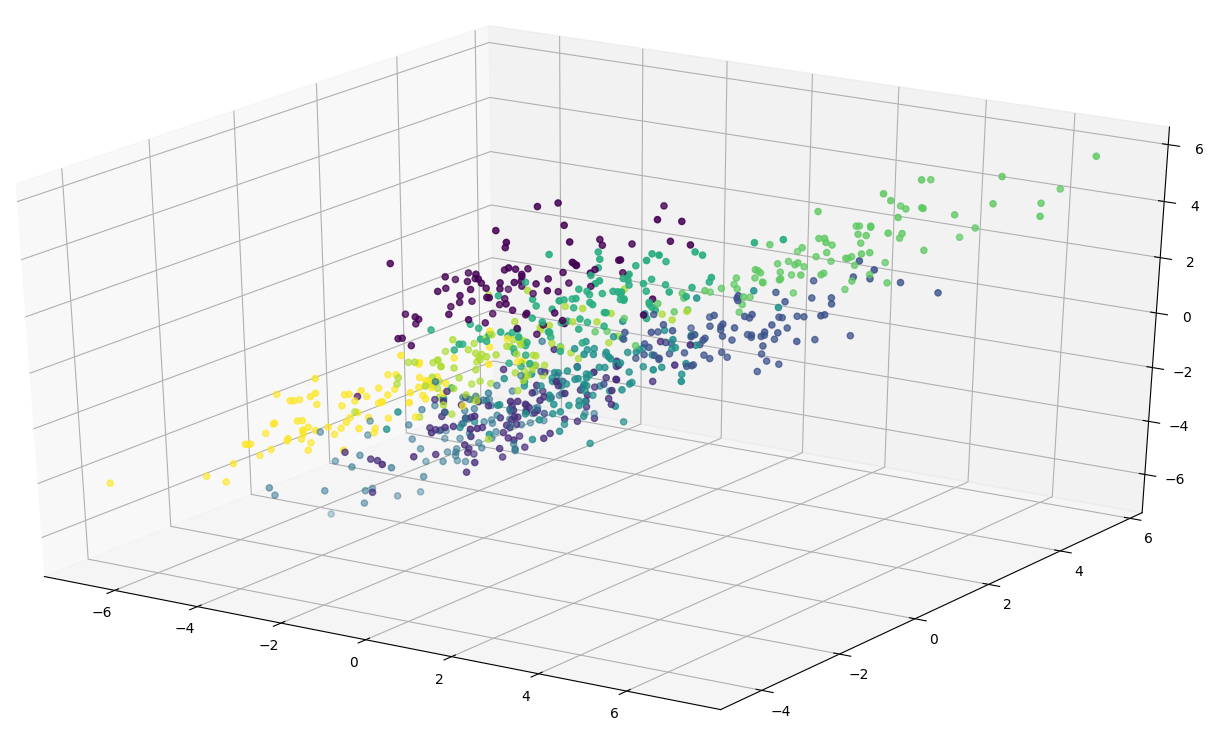
\includegraphics[width=1\linewidth, scale=1]{../img/ej1/sanger_corrida_200_9/sanger_9salida_200ep_testing_dim123.png}
  \caption{Sanger - 9 dimensiones - 200 épocas - Coordenadas 123}
  \label{fig:sub1}
\end{subfigure}%
\begin{subfigure}{.5\textwidth}
  \centering
  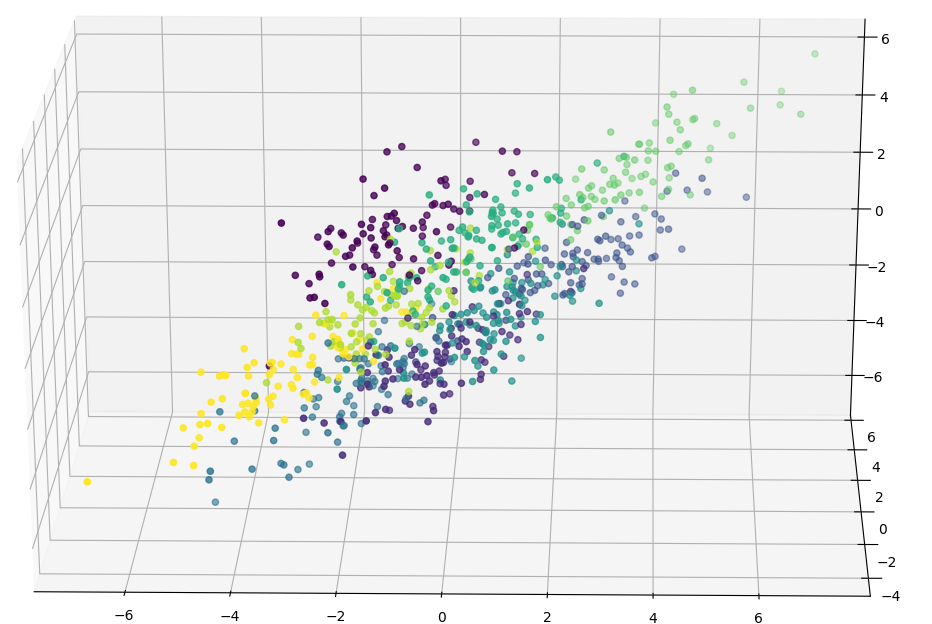
\includegraphics[width=1\linewidth, scale=1]{../img/ej1/sanger_corrida_200_9/sanger_9salida_200ep_testing_dim123_2.png}
  \caption{Sanger - 9 dimensiones - 200 épocas - Coordenadas 123}
  \label{fig:sub2}
\end{subfigure}
\end{figure}

\begin{figure}[!htbp]
\centering
\begin{subfigure}{.5\textwidth}
  \centering
  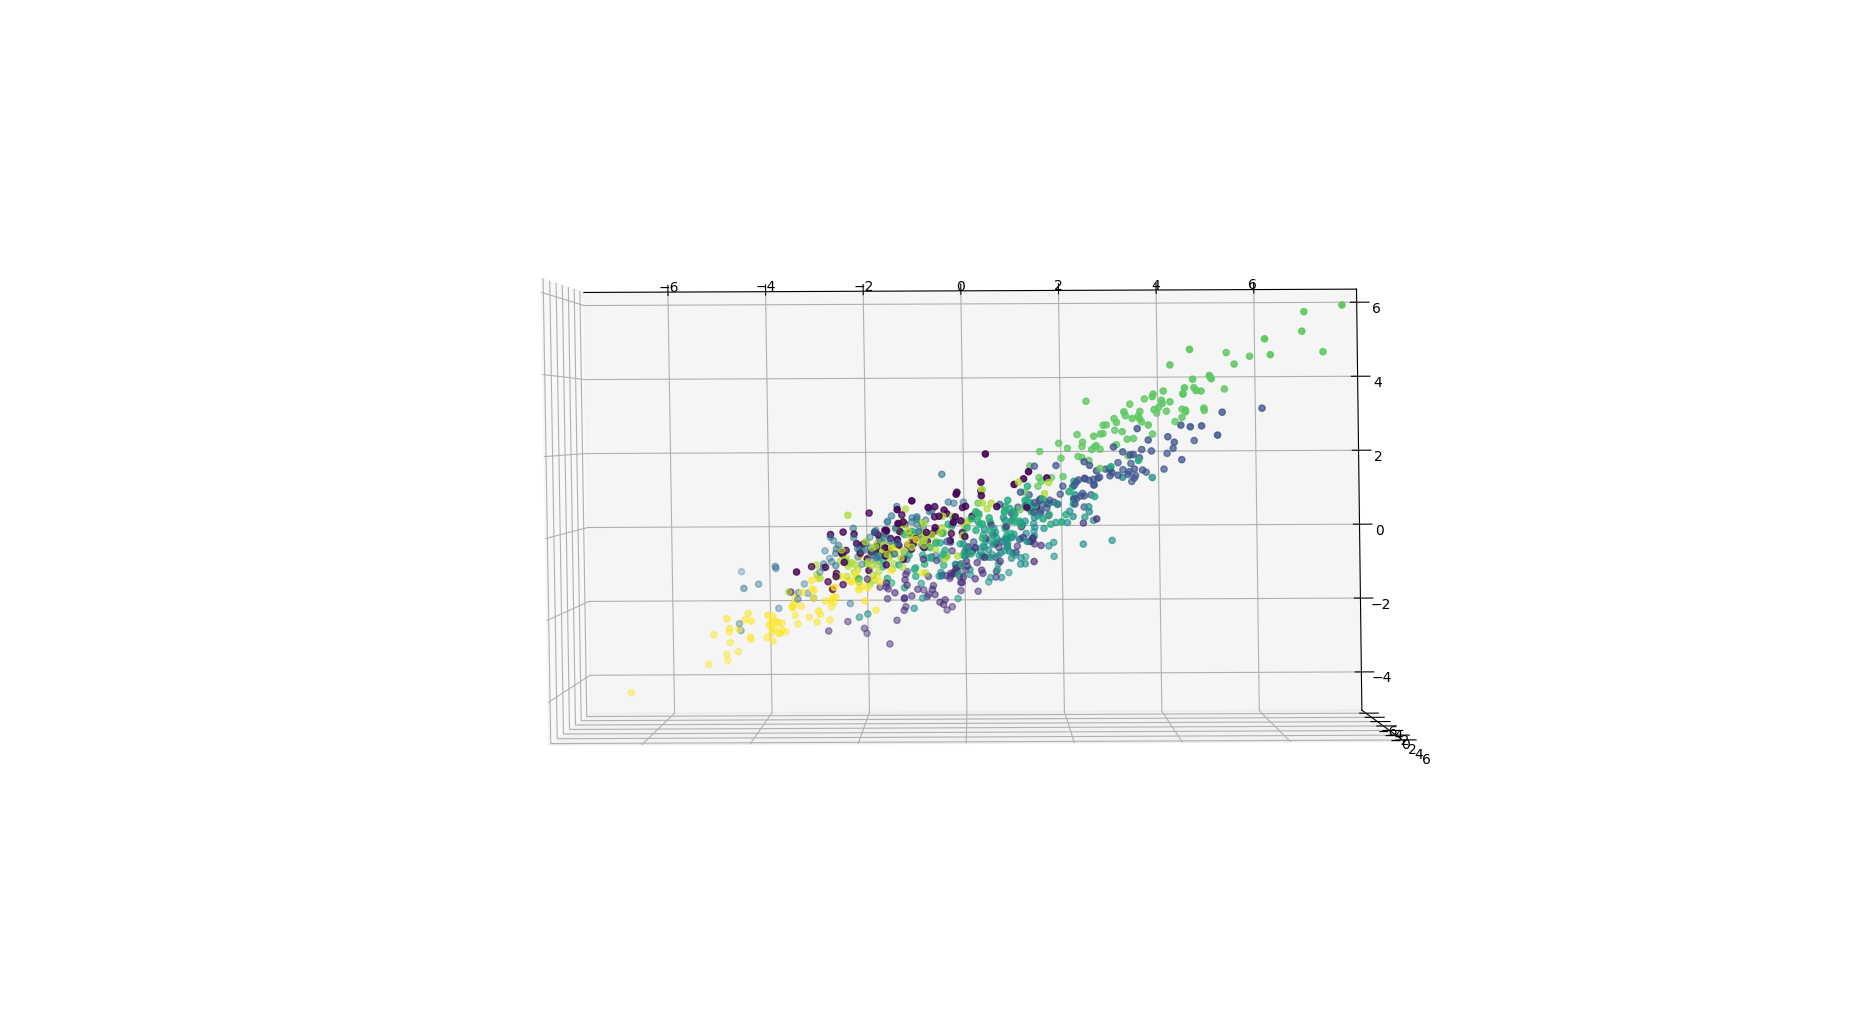
\includegraphics[width=1\linewidth, scale=1]{../img/ej1/sanger_corrida_200_9/sanger_9salida_200ep_testing_dim123_3.png}
  \caption{Sanger - 9 dimensiones - 200 épocas - Coordenadas 123}
  \label{fig:sub1}
\end{subfigure}%
\begin{subfigure}{.5\textwidth}
  \centering
  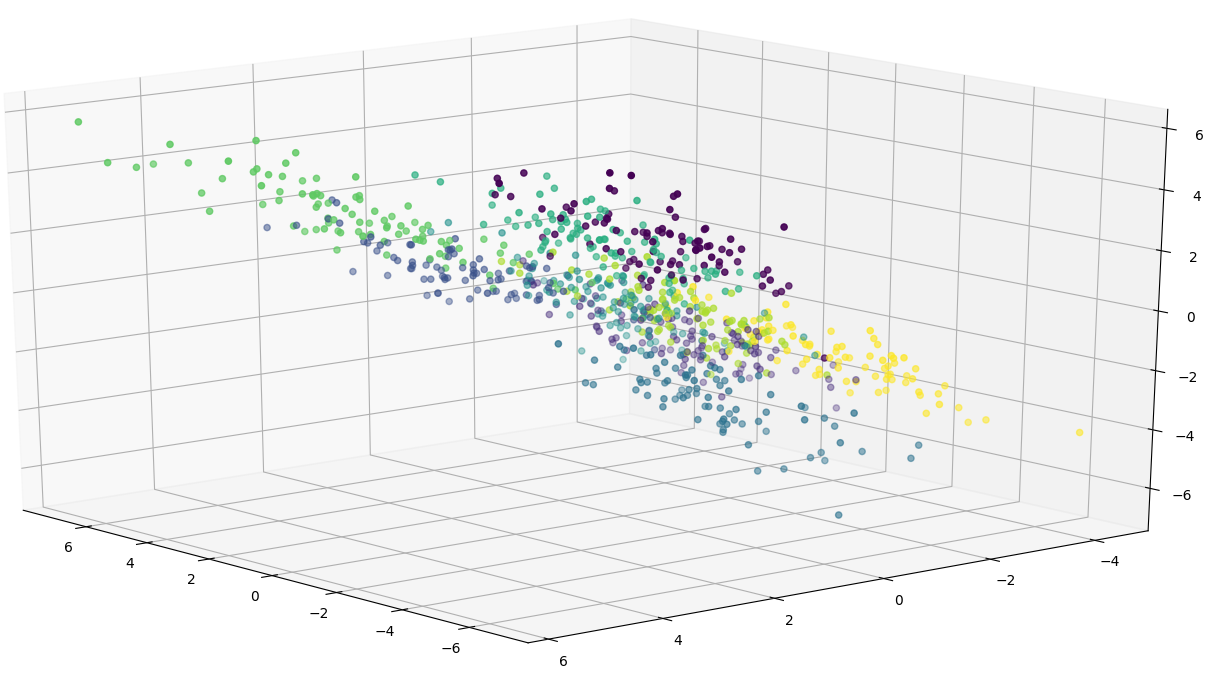
\includegraphics[width=1\linewidth, scale=1]{../img/ej1/sanger_corrida_200_9/sanger_9salida_200ep_testing_dim123_4.png}
  \caption{Sanger - 9 dimensiones - 200 épocas - Coordenadas 123}
  \label{fig:sub2}
\end{subfigure}
\end{figure}

Usando la regla de Sanger se observan mucho mejores resultados. Se pueden observar los clusters separados con mucha mayor claridad. 

A continuación los resultados de las coordenadas 456:

\begin{figure}[!htbp]
\centering
\begin{subfigure}{.5\textwidth}
  \centering
  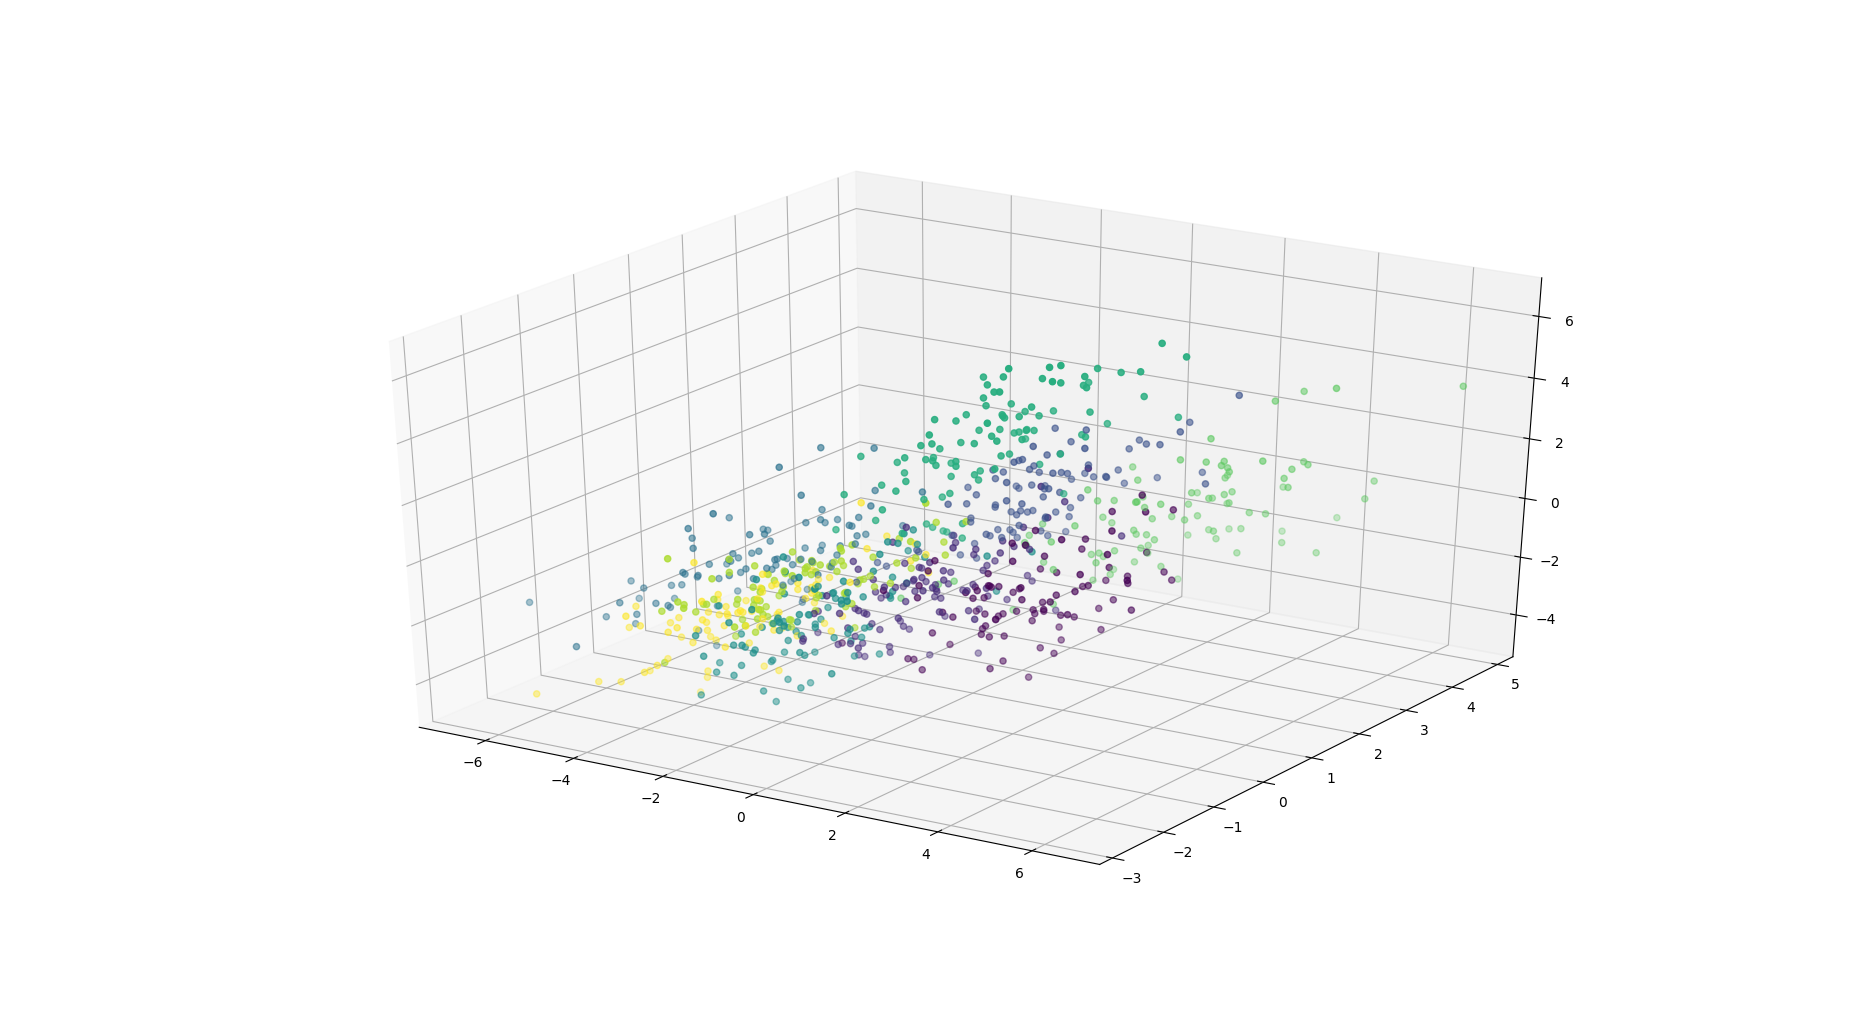
\includegraphics[width=1\linewidth, scale=1]{../img/ej1/sanger_corrida_200_9/sanger_9salida_200ep_testing_dim456.png}
  \caption{Sanger - 9 dimensiones - 200 épocas - Coordenadas 456}
  \label{fig:sub1}
\end{subfigure}%
\begin{subfigure}{.5\textwidth}
  \centering
  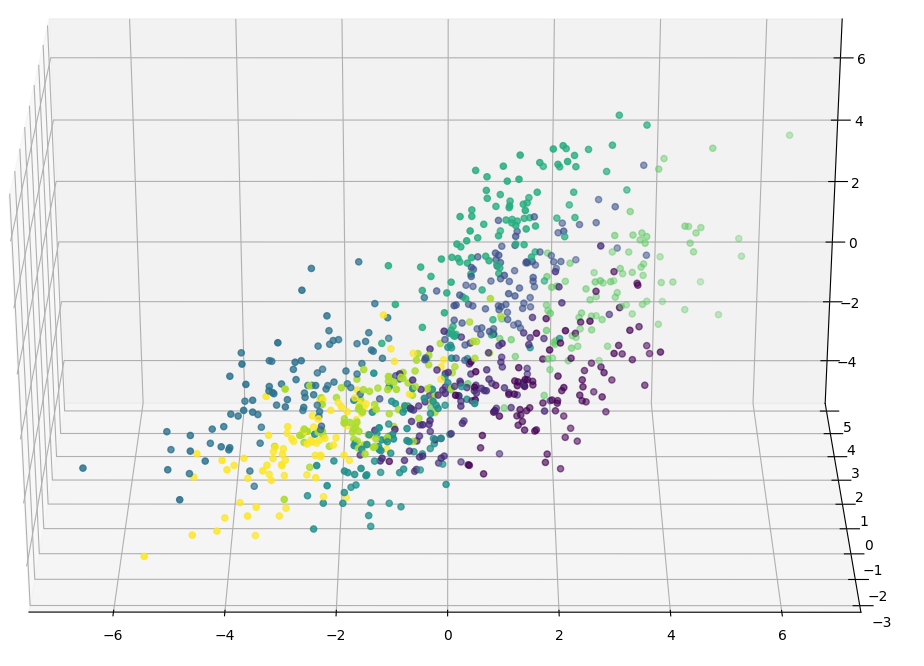
\includegraphics[width=1\linewidth, scale=1]{../img/ej1/sanger_corrida_200_9/sanger_9salida_200ep_testing_dim456_2.png}
  \caption{Sanger - 9 dimensiones - 200 épocas - Coordenadas 456}
  \label{fig:sub2}
\end{subfigure}
\end{figure}

\begin{figure}[!htbp]
\centering
\begin{subfigure}{.5\textwidth}
  \centering
  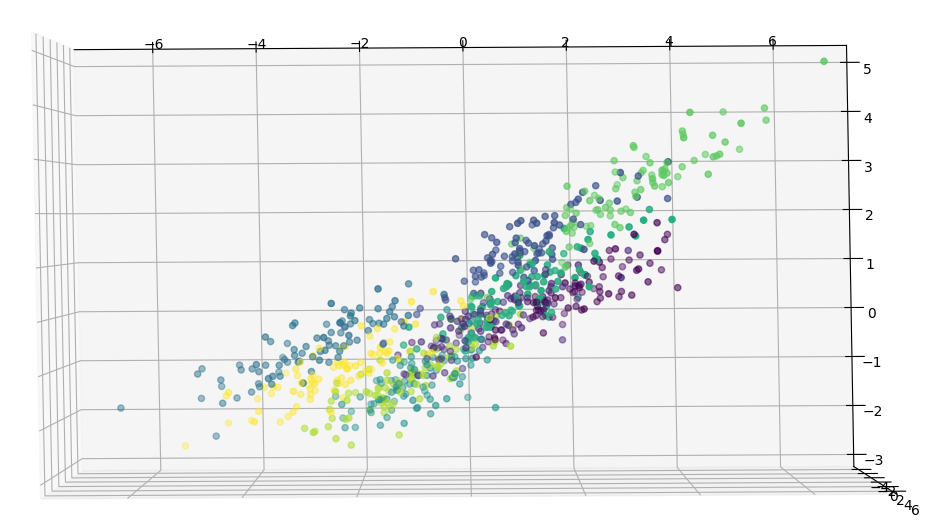
\includegraphics[width=1\linewidth, scale=1]{../img/ej1/sanger_corrida_200_9/sanger_9salida_200ep_testing_dim456_3.png}
  \caption{Sanger - 9 dimensiones - 200 épocas - Coordenadas 456}
  \label{fig:sub1}
\end{subfigure}%
\begin{subfigure}{.5\textwidth}
  \centering
  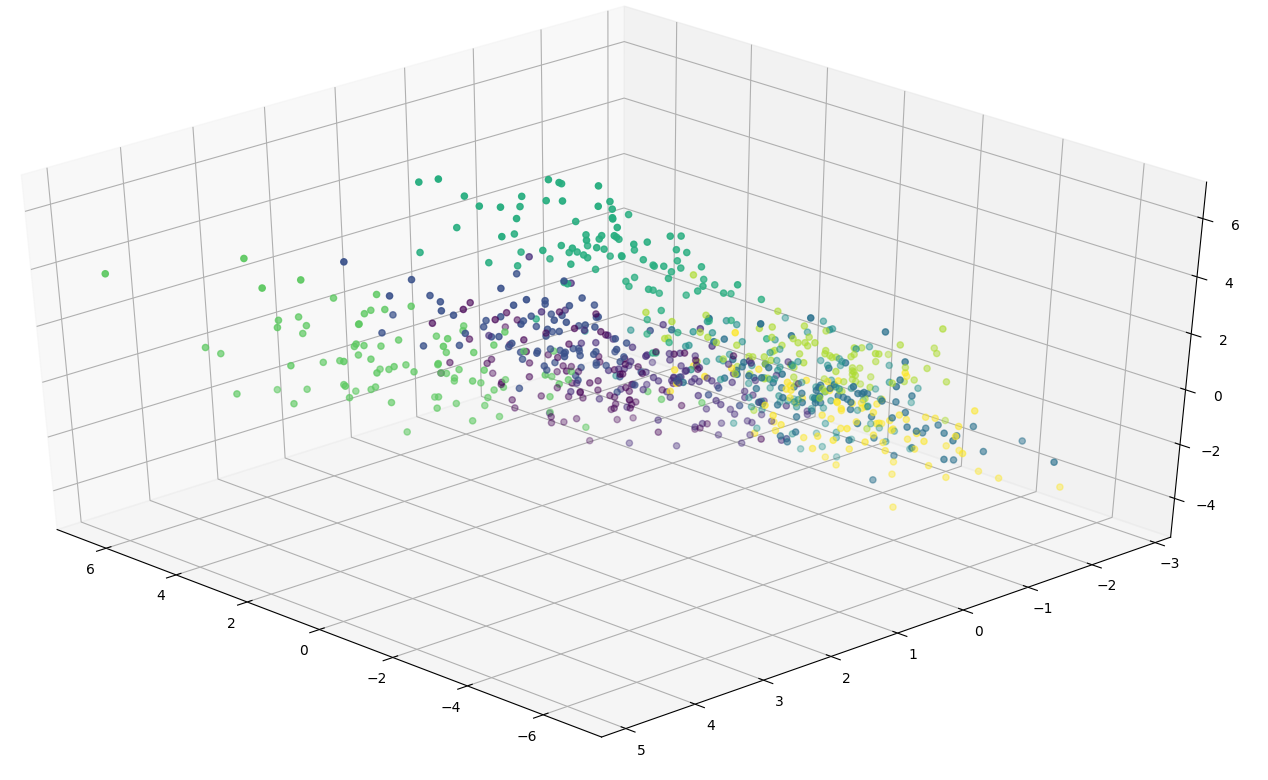
\includegraphics[width=1\linewidth, scale=1]{../img/ej1/sanger_corrida_200_9/sanger_9salida_200ep_testing_dim456_4.png}
  \caption{Sanger - 9 dimensiones - 200 épocas - Coordenadas 456}
  \label{fig:sub2}
\end{subfigure}
\end{figure}

En esta tanda vemos nuevamente una clasificación más marcada y con mayor espacio entre los clusters. Se puede apreciar la agrupación
de las marcas del mismo color, mostrando la asociación entre documentos de la misma categoría.

Veamos las últimas 3 coordenadas.


\begin{figure}[!htbp]
\centering
\begin{subfigure}{.5\textwidth}
  \centering
  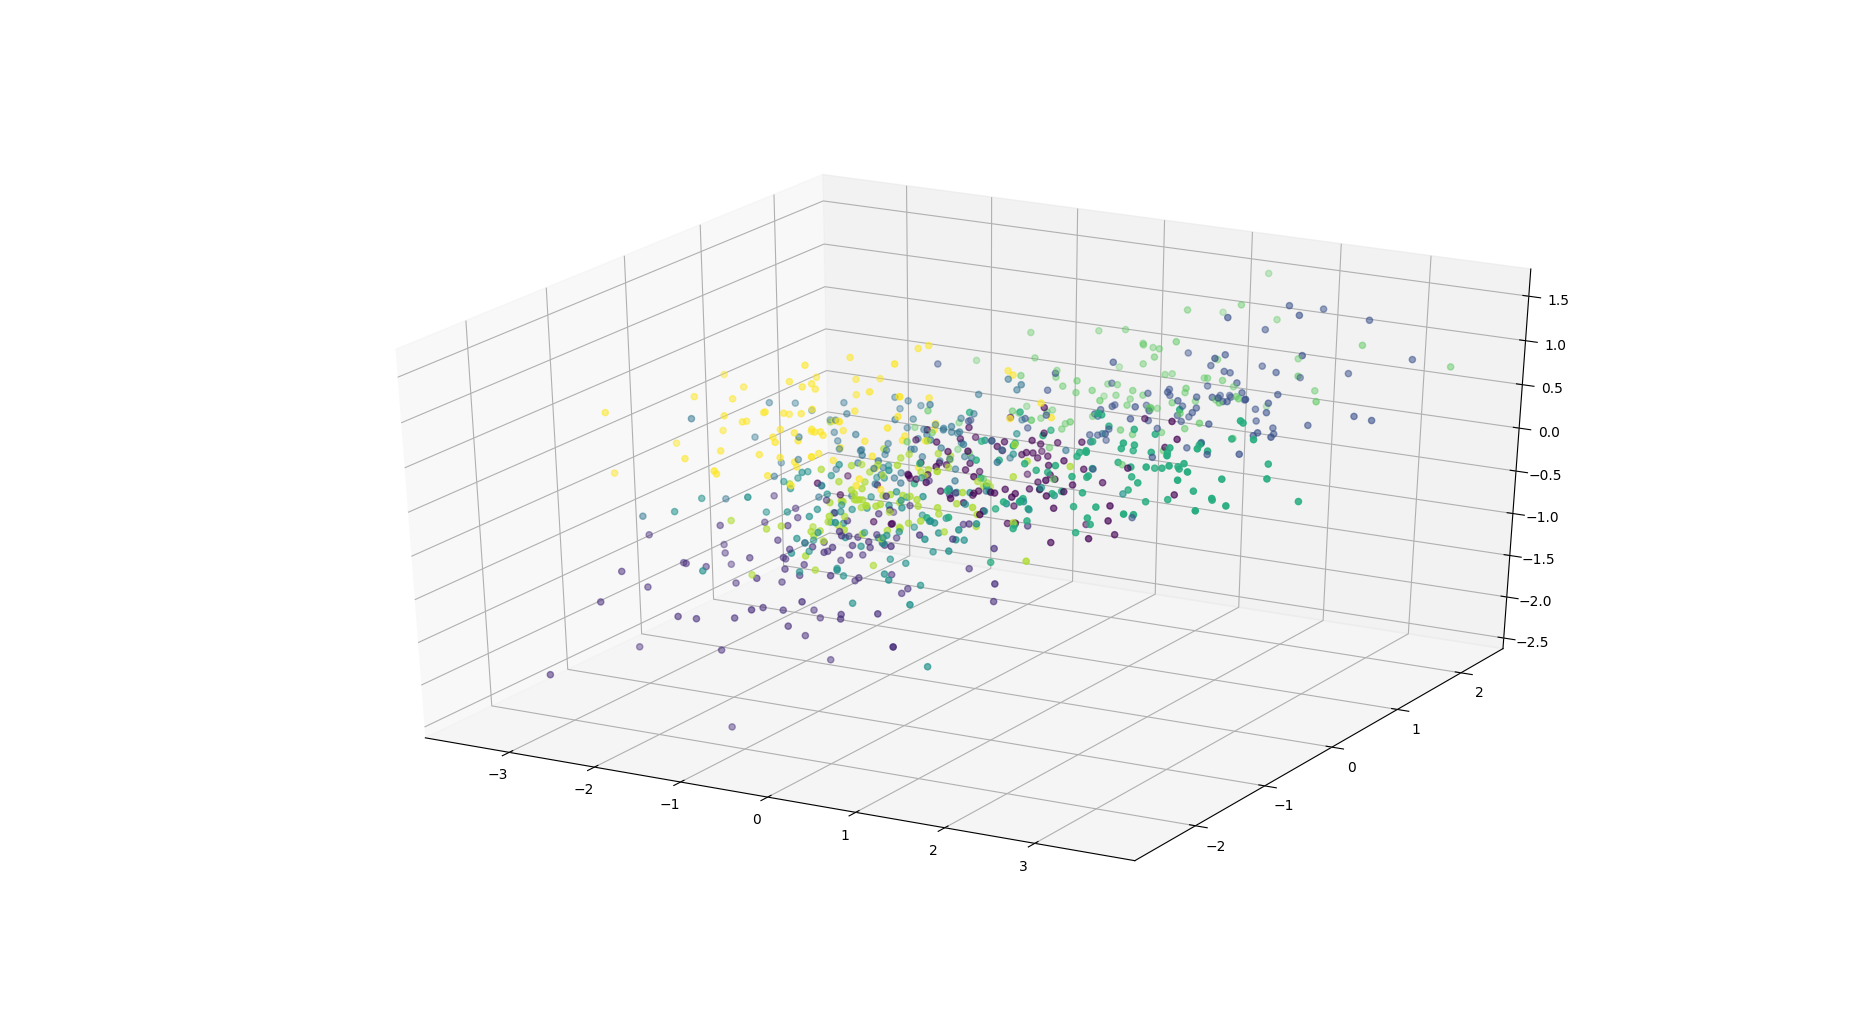
\includegraphics[width=1\linewidth, scale=1]{../img/ej1/sanger_corrida_200_9/sanger_9salida_200ep_testing_dim789.png}
  \caption{Sanger - 9 dimensiones - 200 épocas - Coordenadas 789}
  \label{fig:sub1}
\end{subfigure}%
\begin{subfigure}{.5\textwidth}
  \centering
  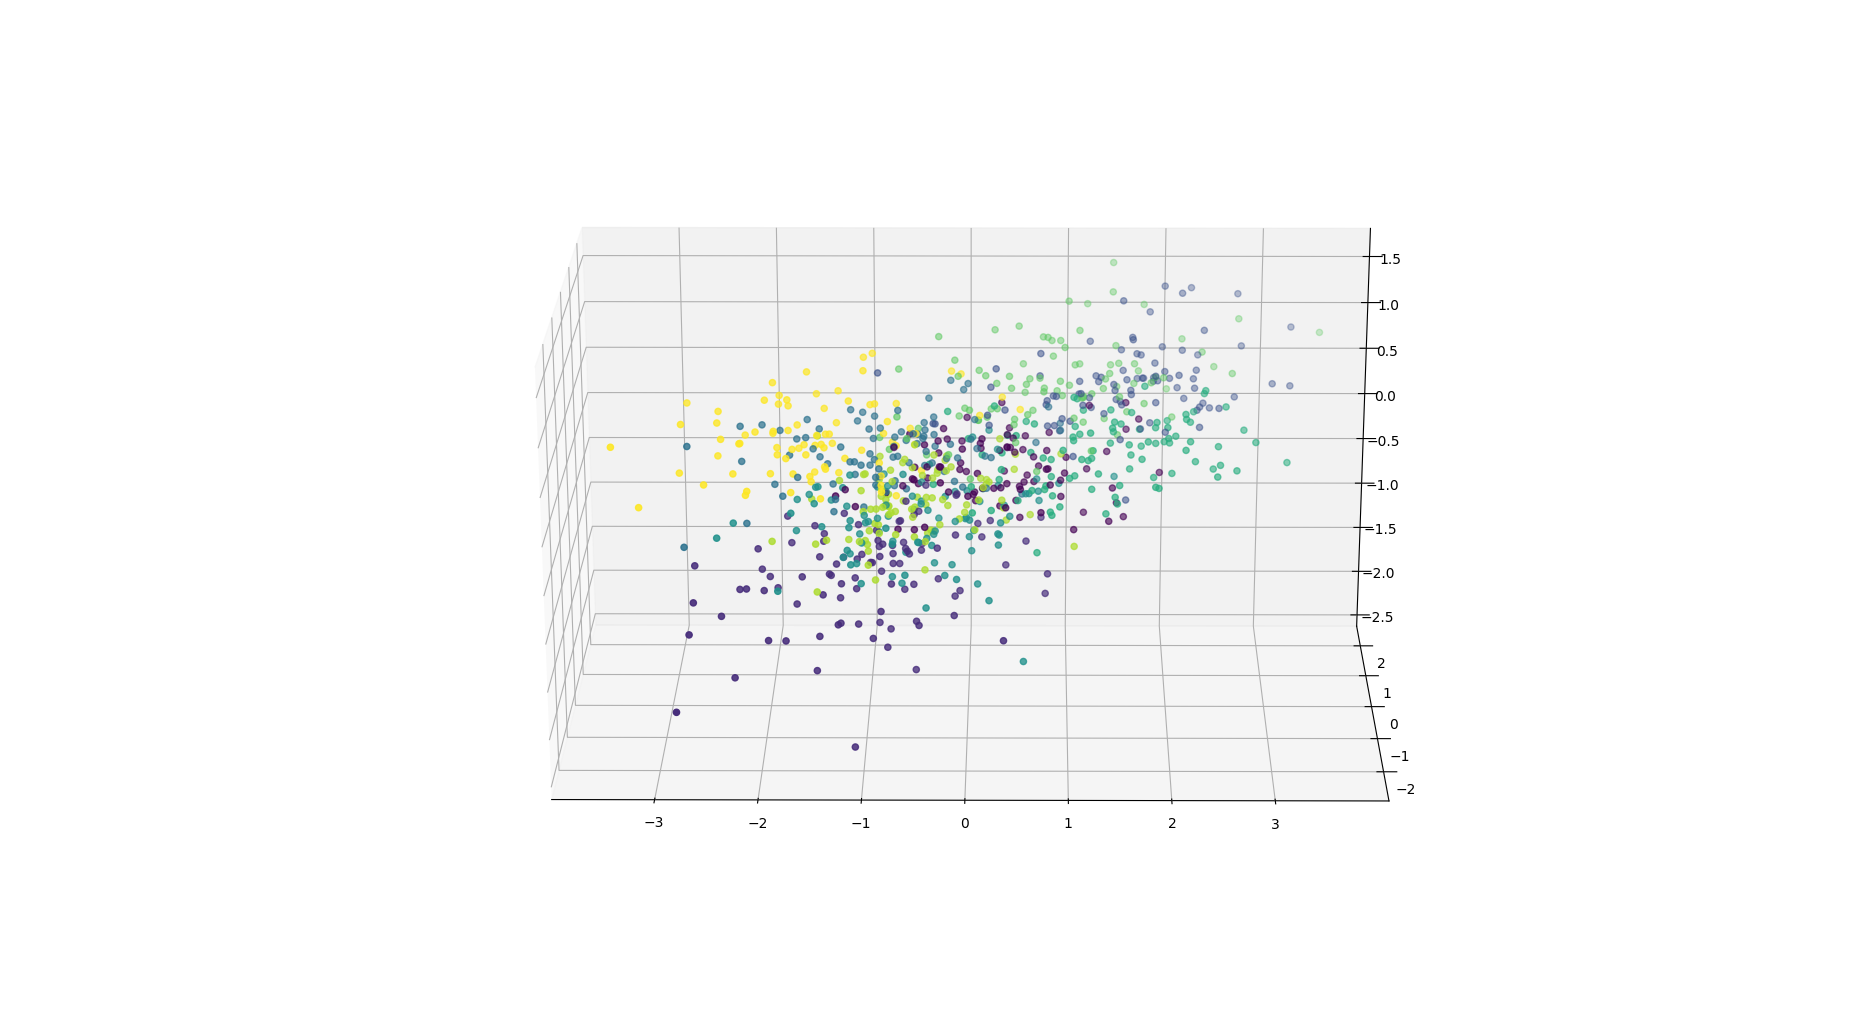
\includegraphics[width=1\linewidth, scale=1]{../img/ej1/sanger_corrida_200_9/sanger_9salida_200ep_testing_dim789_2.png}
  \caption{Sanger - 9 dimensiones - 200 épocas - Coordenadas 789}
  \label{fig:sub2}
\end{subfigure}
\end{figure}

\begin{figure}[!htbp]
\centering
\begin{subfigure}{.5\textwidth}
  \centering
  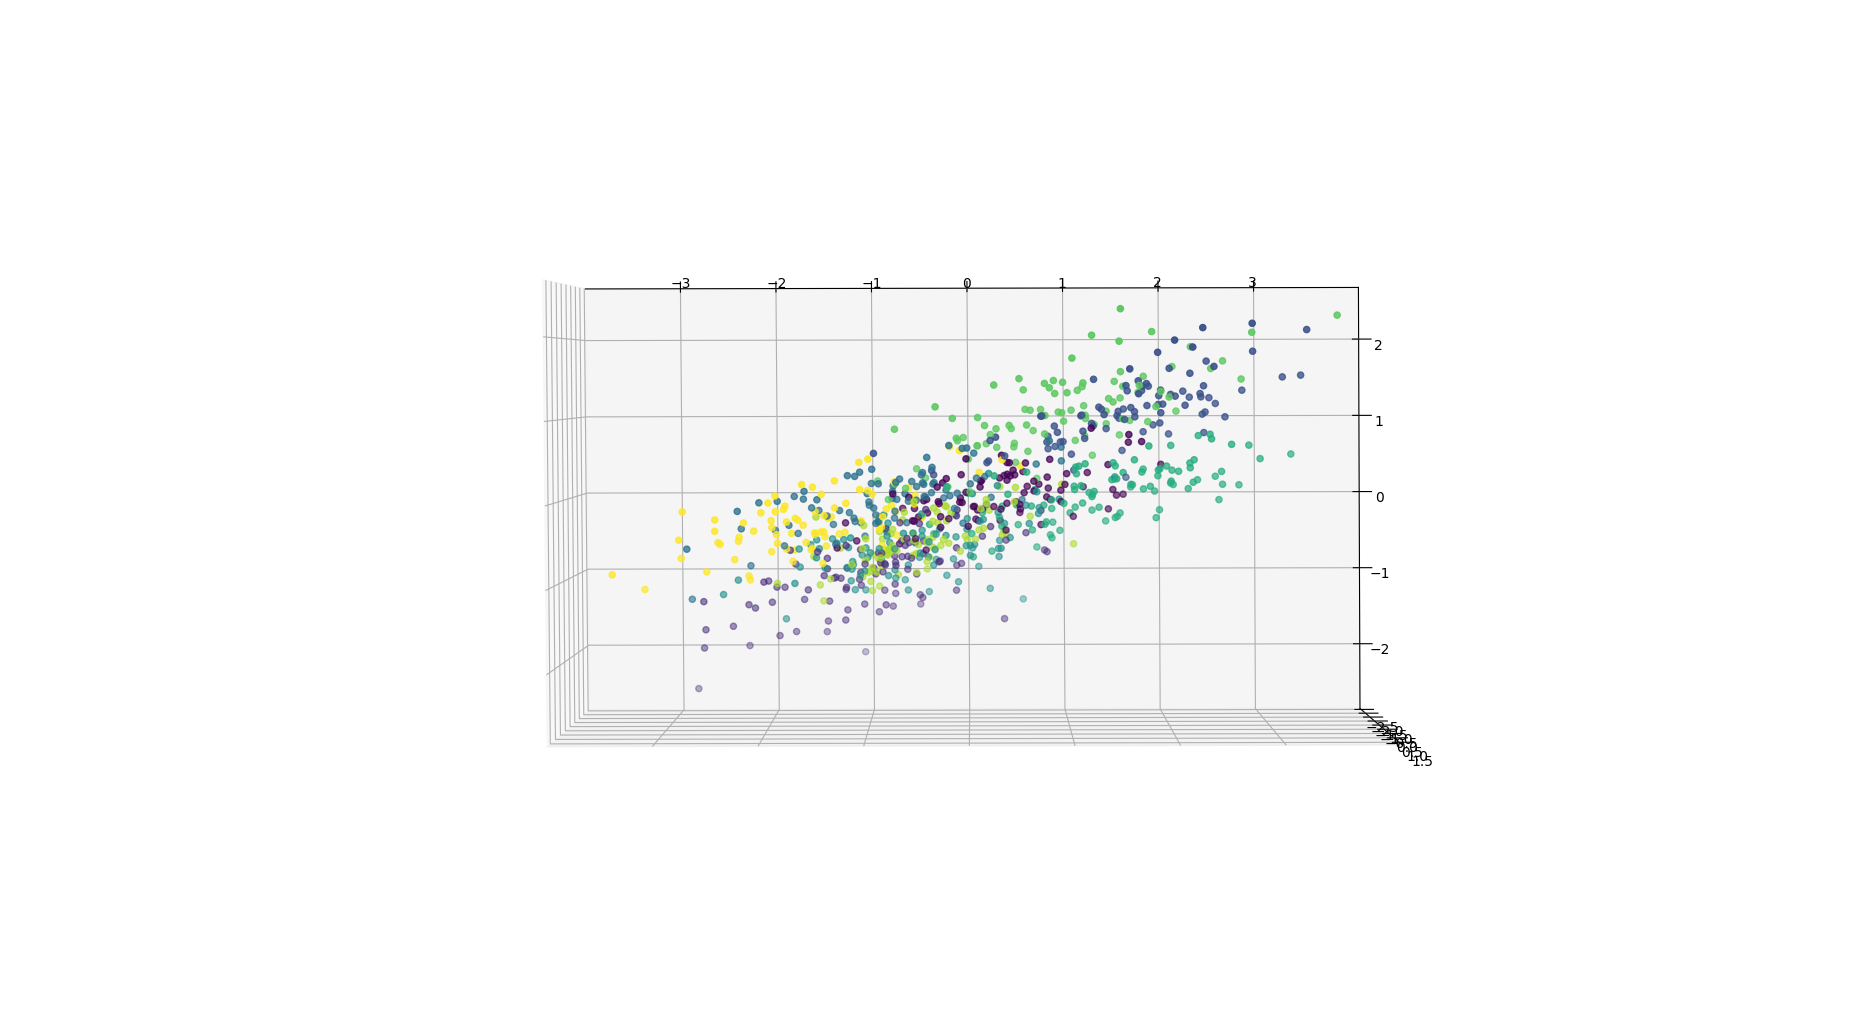
\includegraphics[width=1\linewidth, scale=1]{../img/ej1/sanger_corrida_200_9/sanger_9salida_200ep_testing_dim789_3.png}
  \caption{Sanger - 9 dimensiones - 200 épocas - Coordenadas 789}
  \label{fig:sub1}
\end{subfigure}%
\begin{subfigure}{.5\textwidth}
  \centering
  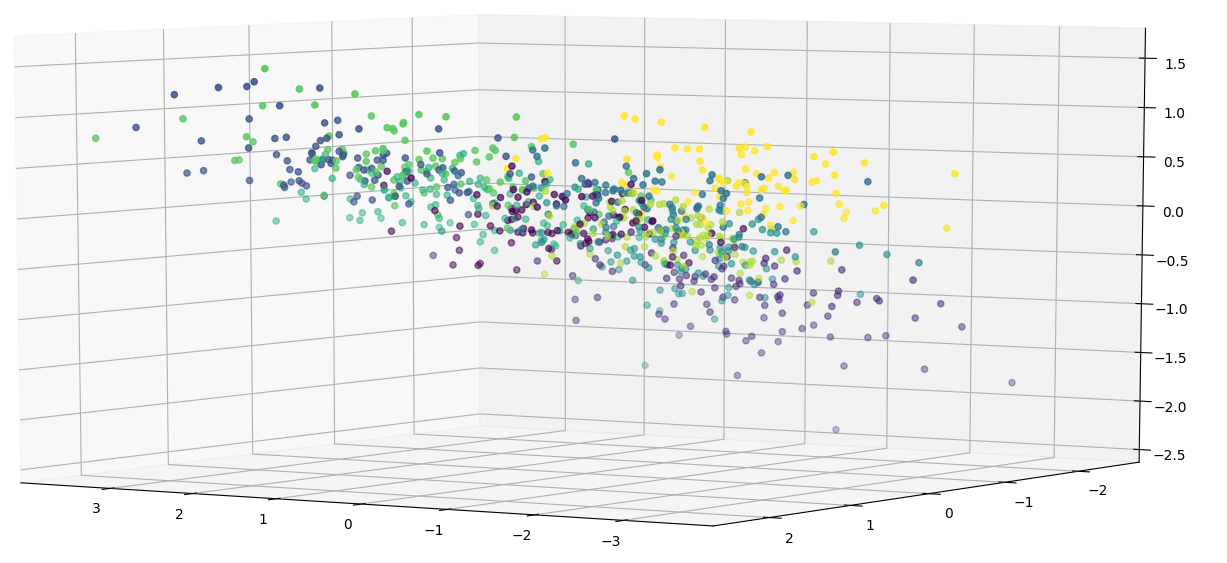
\includegraphics[width=1\linewidth, scale=1]{../img/ej1/sanger_corrida_200_9/sanger_9salida_200ep_testing_dim789_4.png}
  \caption{Sanger - 9 dimensiones - 200 épocas - Coordenadas 789}
  \label{fig:sub2}
\end{subfigure}
\end{figure}

En estas últimas se nota menos precisión en los clusters y mayor solapamiento. Sin embargo, considerado lo observado con Sanger en las primeras 3 coordenadas, éstos son los mejores
resultados que obtuvimos en todo el ejercicio 1. En el caso de esta regla, la ampliación a 9 dimensiones mostró una diferencia notable en la calidad de la solución.

\newpage
\subsection{Ejercicio 2 - Mapeo de características}

Para el segundo ejercicio, los experimentos consistieron en variar la cantidad de neuronas del mapa que podían ser activadas, en conjunto con la cantidad de épocas y la división de las mismas en ordenamiento y convergencia. Intentamos variar estos factores y observar diferencias en los gráficos de estilo mapa de calor generados en base a las categorías que activaron en mayor medida a cada una de las neuronas del mapa.

Comenzamos realizando clasificaciones con 200 épocas como el primer ejercicio, pero, si bien se pudieron apreciar algunos agrupamientos, no fueron lo suficientemente claros. Dado que la performance era bastante más rápida que en el primer ejercicio, decidimos subir las épocas a 1000 como se propuso en clase. Allí observamos una clasificación mejor, con agrupamientos bien definidos.

Estas pruebas fueron hechas tanto para el mapeo de los documentos directamente (donde cada neurona del mapa tiene 850 vectores de entrada), como para las 3 y 9 componentes principales que se obtienen de las redes generadas en el primer ejercicio. Para estos dos últimos casos, utilizaremos las redes generadas con el algoritmo de Sanger, dado que fue el que nos devolvió los mejores resultados.

Finalmente, comparamos los resultados obtenidos entre las 3 opciones para dar nuestra visión de cual funcionó mejor en base a nuestros experimentos.

\subsubsection{Mapeo de documentos con 850 atributos}

En primera instancia, planteamos un experimento utilizando 200 épocas. Como mencionamos anteriormente, esta cantidad de épocas no produjo buenos resultados. En consecuencia, aumentamos la cantidad a 1000 como se mencionó en clase. Decidimos tomar un mapa de neuronas de 10 x 10 como primera prueba. Nos pareció un buen número para empezar para darle oportunidad a cada neurona de que sea activada por más de un documento (810 documentos de entrenamiento sobre 100 neuronas del mapa). 

\begin{figure}[h]
  \begin{center}
    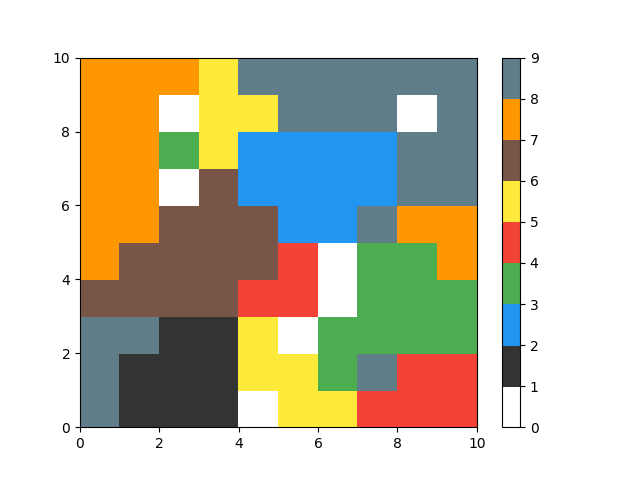
\includegraphics[scale=0.6]{../img/map_1000ep_850en.png}
  \caption{Mapa 10x10 - 850 ejes x neurona - 1000 épocas - Sigma 5 - Entrenamiento}
  \end{center}
\end{figure}

Si bien hay un idea de agrupamiento, éste no es tan claro como esperábamos, por lo cual decidimos variar el parámetro T1 del cálculo del sigma inicial para que la función logaritmo del sigma que nosotros pasamos por parámetro le aplique logaritmo en base 2 en vez de logaritmo natural. Luego, volvimos a correr el experimento y obtuvimos mejores resultados. Observemos:
\newpage

\begin{figure}[h]
  \begin{center}
    \includegraphics[scale=0.6]{../img/map_1000ep_850en_v2.png}
  \caption{Mapa 10x10 - 850 ejes x neurona - 1000 épocas - Sigma 5 - Entrenamiento}
  \end{center}
\end{figure}

Encontramos muy extraño que haya tantos blancos en el mapa. Cada uno indica que esas neuronas no fueron activadas por ningún documentoal realizar la última recorrida de los documentos sobre la red entrenada para armar el mapa. Esto nos desconcertó, por lo que recurrimos a consultarlo con los profesores. Entendimos que esto no debería suceder y que las posibles causas podían ser que nuestro mapa era demasiado grande, o que teníamos algún problema en la función de vecindad y/o las fases de ordenamiento y convergencia y/o nuestro código en sí.

Luego de revisar nuestra implementación, descubrimos que las fases de ordenamiento y convergencia no estaban muy bien definidas y que durante todas las épocas tanto el sigma como el eta no dejaban de ser \textit{enfriados}. Es por eso que decidimos plantear que de las 1000 épocas, dos tercios de las mismas fueran de ordenamiento y el resto de convergencia. Además, decidimos achicar el área de nuestro mapa de neuronas de 10x10 a 8x8 y volvimos a correr el experimento con sigma 5 y con sigma 8.

\begin{figure}[!htbp]
\centering
\begin{subfigure}{.5\textwidth}
  \centering
  \includegraphics[width=1\linewidth, scale=1]{../img/map8x8_1000ep_850en.png}
  \caption{Mapa 8x8 - 850 ejes x neurona - 1000 épocas - Sigma 5 - Entrenamiento}
  \label{fig:sub1}
\end{subfigure}%
\begin{subfigure}{.5\textwidth}
  \centering
  \includegraphics[width=1\linewidth, scale=1]{../img/map8x8_1000ep_850en_sigma8.png}
  \caption{Mapa 8x8 - 850 ejes x neurona - 1000 épocas - Sigma 8 - Entrenamiento}
  \label{fig:sub2}
\end{subfigure}
\end{figure}

Con los resultados podemos ver que la presencia de blancos disminuyó ligeramente pero siguen presentes. También podemos notar que no se obtiene una clusterización perfecta que es lo que quisimos lograr. Debido a que no estar conformes con éstos resultados, decidimos modificar la duración de las fases de ordenamiento y convergencia. Recordemos que hasta este momento estábamos utilizando dos tercios de la 1000 épocas para el ordenamiento y el tercio restante para convergencia (~333 épocas para convergencia). Ahora, en vez de eso, haremos pruebas con 1 medio (500 épocas) y 1 cuarto (250 épocas) para convergencia.

\newpage

\begin{figure}[!htbp]
\centering
\begin{subfigure}{.5\textwidth}
  \centering
  \includegraphics[width=1\linewidth, scale=1]{../img/map8x8_1000ep_850en_sigma8_faseord500.png}
  \caption{Mapa 8x8 - 850 ejes x neurona - 1000 épocas (500 ord/500 conv) - Sigma 8 - Entrenamiento}
  \label{fig:sub1}
\end{subfigure}%
\begin{subfigure}{.5\textwidth}
  \centering
  \includegraphics[width=1\linewidth, scale=1]{../img/map8x8_1000ep_850en_sigma8_faseord750.png}
  \caption{Mapa 8x8 - 850 ejes x neurona - 1000 épocas (750 ord/250 conv) - Sigma 8 - Entrenamiento}
  \label{fig:sub2}
\end{subfigure}
\end{figure}

Como se puede apreciar, el problema de clusterización se resuelve mucho mejor utilizando 750 épocas para el ordenamiento y 250 para la convergencia. Por otro lado, el problema de los blancos sigue presente, lo cual nos lleva nuevamente a replantear nuestros parámetros para eliminar este comportamiento en su totalidad. Es por eso que decidimos utilizar un mapa de neuronas más pequeño, de 7x7 en vez de 8x8. 

\begin{figure}[!htbp]
  \begin{center}
    \includegraphics[scale=0.6]{../img/map7x7_1000ep_850en_sigma7_faseord750.png}
  \caption{Mapa 7x7 - 850 ejes x neurona - 1000 épocas (750 ord/250 conv) - Sigma 7 - Entrenamiento}
  \end{center}
\end{figure}

Ahora sí, en este experimento conseguimos los resultados esperados, con lo cual confirmamos que nuestro problema era que el mapa de neuronas estaba demasiado grande. Un detalle importante es que luego de realizar este experimento nos dimos cuenta que las categorías 8 y 9 estaban siendo coloreadas de la misma manera, con lo cual tuvimos que ajustar el mapa para que salga correctamente.

\newpage

\begin{figure}[!htbp]
  \begin{center}
    \includegraphics[scale=0.6]{../img/map7x7_1000ep_850en_sigma7_faseord750_corregido.png}
  \caption{Mapa 7x7 - 850 ejes x neurona - 1000 épocas (750 ord/250 conv) - Sigma 7 - Entrenamiento}
  \end{center}
\end{figure}

Hicimos también pruebas variando el ancho del mapa de neuronas para, en vez de tener un mapa cuadrado, sea rectangular. En este caso, intentamos con mapas de 7x6, 7x8 y 7x9. Sin embargo, no obtuvimos mejores clusterizaciones que con el de 7x7.

Finalmente, para el mapa de 7x7, calculamos el error de predicción de categoría del mismo utilizando los datos de validación. O sea, para cada uno de los documentos que seleccionamos para validación, chequeamos cual es la neurona que más activa y comparamos la categoría que más activa esa neurona con la categoría del documento (de validación) que estamos chequeando. Por cada diferencia de categoría entre el documento validado y la categoría que más activa la neurona, la contamos para luego mostrarla en el gráfico.

\begin{figure}[!htbp]
  \begin{center}
    \includegraphics[scale=0.6]{../img/map7x7_1000ep_850en_sigma7_faseord750_corregido_errores.png}
  \caption{Cantidad de errores por categoría. $X=$: categorías, $Y=$ cantidad de errores.}
  \end{center}
\end{figure}

Como se puede apreciar, la categorización es excelente, todos los documentos de nuestro conjunto de validación mapean a neuronas que se corresponden con su categoría, que era nuestro objetivo para esta tipo de red.

Tiempo de ejecución: ~750 segundos.

\subsubsection{Mapeo de documentos con 3 componentes principales}

En este experimento, en lugar de utilizar los 850 atributos de cada documento para hacer el mapeo con nuestro mapa de neuronas, aprovechamos las redes generadas en el ejercicio 1 para obtener las componentes principales de cada uno de los documentos. Luego, utilizamos estas componentes como entrada de las neuronas de nuestro mapa, y de esta manera comparamos los resultados con los obtenidos en la sección anterior. Replicamos el experimento utilizando reducciones de 3 y 9 dimensiones.

Para poder generar la entrada, utilizamos dos redes entrenadas, las cuales incluimos en el TP:\\ \textbf{sanger200\_dim3.json} y \textbf{sanger200\_dim9.json}. Corresponden a redes entrenadas con regla de Sanger y que calculan reducción a 3 y 9 componentes principales. En ellas se utilizaron 200 épocas de training ya que fue la cantidad óptima concluída de los experimentos.

Fijamos el resto de los parámetros de la prueba con los valores óptimos de la sección anterior: 1000 épocas de entrenamiento, Sigma 7, mapa de 7x7.\\

Observemos primero los resultados, utilizando 3 componentes princiales como entrada:

\begin{figure}[!htbp]
  \begin{center}
    \includegraphics[scale=0.6]{../img/map7x7_1000ep_3en_sigma7_faseord750.png}
  \caption{Mapa 7x7 - 3 componentes de entrada - 1000 épocas (750 ord/250 conv) - Sigma 7 - Entrenamiento}
  \end{center}
\end{figure}

El mapa obtenido es bastante aceptable. Se pueden apreciar los distintos clusters con claridad. Hay un par de categorías que se encuetran dispersas como la 5, la 6 y la 8.
Podemos ver que la calidad del mapa no es tan buena como la obtenida utilizando la totalidad de los atributos.

Este mapa aquí exhibido se generó con los datos de entrenamiento, utilizando el 90\% del dataset. Para poder medir la capacidad de generalizar de la red: se usaron los documentos restantes  como datos de validación y sobre éstos calculamos cuantos errores de clasificación se obtuvieron. 

Veamos la cantidad de errores por categoría:

\newpage

\begin{figure}[!htbp]
  \begin{center}
    \includegraphics[scale=0.45]{../img/validation_1000ep_3en_sigma7_faseord750.png}
  \caption{Cantidad de errores por categoría. $X=$: categorías, $Y=$ cantidad de errores.}
  \end{center}
\end{figure}

Vemos que a la hora de predecir categorías, esta red presenta muchos más errores que su contraparte de 850 atributos. En aquella no se habían generado errores mientras que aquí, en total, hay más del 30\% de desaciertos, considerando que se clasificaron 90 documentos y hay 34 errores. 

Este resultado es llamativo, ya que esperábamos mayor eficiencia en la generalizacion de documentos nuevos. Creemos que esto se debió a la menor información que presenta la reducción de dimensiones como entrada.

El tiempo de ejecución total con 3 componentes fue de: ~680 segundos.

Veamos si se mantuvo la tendencia utilizando 9 dimensiones.

\subsubsection{Mapeo de documentos con 9 componentes principales}

Este experimento replica al anterior, pero con la entrada del experimento teniendo 9 componentes principales. Todos los demás parámetros fijados en los mismos valores.

Veamos la calidad del mapa obtenido:

\begin{figure}[!htbp]
  \begin{center}
    \includegraphics[scale=0.48]{../img/map7x7_1000ep_9en_sigma7_faseord750.png}
  \caption{Mapa 7x7 - 9 componentes de entrada - 1000 épocas (750 ord/250 conv) - Sigma 7 - Entrenamiento}
  \end{center}
\end{figure}

Observamos que este mapa también tiene buena claridad y separación entre los clusters. Al igual que con 3 componentes, algunas de las categorías se encuentran dispersas, como la 1 y la 8.
Presenta una calidad aceptable, pero no tan buena como la del mapa de 850 atributos.

A continuación los errores de predicción sobre el conjunto de validación:

\begin{figure}[!htbp]
  \begin{center}
    \includegraphics[scale=0.45]{../img/validation_1000ep_9en_sigma7_faseord750.png}
  \caption{Cantidad de errores por categoría. $X=$: categorías, $Y=$ cantidad de errores.}
  \end{center}
\end{figure}

La figura muestra que se mantuvo una tasa alta de errores. Con 32 errores sobre 90 documentos, la capacidad de predicción no es muy buena, manteniendo aproximadamente la misma efectividad que la red del experimento anterior.

Estos resultados nos indican que tomar como entrada menor cantidad de componentes tuvo un impacto negativo sobre la calidad del mapa y especialmente sobre la efectividad de la red para generalizar los datos de validación. Inicialmente creíamos que se iba a mantener una performance relativamente igual de buena pero los resultados nos contradijeron.

El tiempo de ejecución total con 9 componentes fue de: ~721 segundos. Observando los tiempos obtenidos en los experimentos anteriores, no se nota un descenso notable de la performance utilizando menos componentes.

\newpage
\section{Respuestas a preguntas del enunciado}

\subsubsection{Ejercicio 1}

\begin{itemize}

\item \textbf{¿Qué interpretación le puede dar a estos resultados?} 

Lo que podemos interpretar es que tanto el algoritmo de Oja como el de Sanger, logran realizar una clusterización de los documentos según 
su categoría, entrenándose sin saber a priori la categoría de cada documento. Luego con las categorías de cada documento confirmamos esta 
clusterización. Esto significa que los documentos de cada categoría exponen algún tipo de patrón en sus atributos que los permite agrupar en 
diferentes clusters. Como resultado, Oja y Sanger (Sanger en mejor medida) logran crear una red que permite determinar la categoría de nuevos
documentos a partir de sus componentes principales con un buen nivel de precisión.

\item \textbf{¿Qué tan buenos son estos modelos específicos para hacer una clasificación de los documentos?}

Ambos modelos lograron de alguna forma clusterizar los documentos y de ésta manera se pueden diferenciar ciertas áreas del espacio
donde documentos de misma categoría se agrupan. Sanger dio mejores resultados que Oja, y teniendo en cuenta que las áreas en Sanger
están mucho mejor definidas, se podría decir que la clasificación de documentos es bastante buena, e incluso podría mejorar aumentando
las épocas de entrenamiento (si tuviésemos el poder de cómputo adecuado, dado que demora bastante tiempo).

\item \textbf{¿Cómo los utilizaría?}

Una vez que la red está entrenada, podemmos delimitar áreas en el espacio que corresponden a cada categoría. Luego, para nuevos documentos
(o cualquier otro tipo de información que queramos categorizar), solo debemos ver en que área se ubica con sus componentes principales a partir de
eso podemos concluir cual es su categoría con un nivel de precisión bastante bueno que nos da el algoritmo de Sanger.

\end{itemize}

\subsubsection{Ejercicio 2}

\begin{itemize}

\item \textbf{¿Qué interpretación puede darle a los resultados obtenidos?} 

Como se puede apreciar en los resultados de nuestros experimentos, los mapas autoorganizados permiten agrupar y mapear las categorías
de los documentos en las neuronas de nuestro mapa, logrando que neuronas que mapean a mismas categorías sean adyacentes entre sí. Luego de
un extenso entrenamiento dividido en las fases de ordenamiento y convergencia, la red entrenada ofrece un mapa de categoría altamente 
preciso, ya que al validarlo con datos de validación (que no fueron utilizados para entrenar), la precisión de determinación de categoría 
según neurona activada fue del 100\%. Esto nos permite decir que el mapa autoorganizado es un gran método de clasificación, por lo menos para
este caso de clasificación de documentos.

\item \textbf{¿Cómo se comparan estos resultados con los obtenidos anteriormente?}

Se comparan directamente. En ambos ejercicios las redes resultantes nos permiten realizar una categorización de datos nuevos con un buen 
nivel de precisión. Sin embargo, creemos que los mapas autoorganizados facilitan en gran medida la comparación y determinación de categoría 
para nuevos datos ya que es mucho más directa debido a las 2-dimensionalidad del mapa contra la 3/9-dimensionalidad de las componentes principales, 
para las cuales deberíamos delimitar áreas en esas dimensiones para saber si las componentes de nuevos documentos caen dentro de cuales áreas para 
determinar su categoría.

\item \textbf{¿Cuál es la arquitectura de red y parámetros de entrenamiento que utilizaría?}

Luego de toda la experimentación realizadas, concluimos que la mejor configuración para realizar el entrenamiento de 
la red es la siguiente:

\begin{itemize}
\item Tamaño de mapa de neuronas: 7 x 7
\item Sigma inicial: 7
\item Eta inicial: 0.1
\item Épocas totales: 1000
\item Duración ordenamiento: 750 épocas
\item Duración convergencia: 250 épocas
\item Tipos de datos de entrada: datos en bruto (850 atributos por documento)
\end{itemize}

\item \textbf{¿Qué resultados esperaría obtener con datos de testeo con los que el modelo no fue entrenado?}

Dado que seleccionamos solo el 90\% del conjunto de documentos para hacer el entrenamiento, el otro 10\% restante no fue utilizado 
para entrenar el modelo, y dado que lo utilizamos para calcular el error de categorización del mismo contra la red ya entrenada, 
podemos responder esta pregunta diciendo que se esperaría, que la categorización de estos datos de testeo sea correcta en el 
~97\% de los casos (realizamos experimentos en donde hemos encontrado 1 o 2 errores como máximo luego del entrenamiento, pero la 
mayoría de las veces ninguno).

\item \textbf{¿Hubo diferencia en el tiempo de entrenamiento utilizando los datos de dimensión reducida?}

Sí la hubo, aunque fue bastante reducida, 30 segundos más rápido usar 9 componentes principales contra los 850 atributos, y 70 segundos 
más rápido usar 3 componentes contra los 850 atributos. 

\item \textbf{¿Y en la calidad del resultado?}

En la calidad del resultado, por el contrario, tomar las componentes principales dio resultados muy pobres comparado con 
tomar los 850 atributos de cada documento. Si bien con 3 y 9 componentes principales el mapeo tiene una noción de clusterización,
la cantidad de errores de categorización del conjunto de validación llega a estar por encima del 35\%, lo cual es bastante malo y
resulta en una categorización en la que no se puede confiar. 

\end{itemize}

\section{Conclusión}

En toda nuestra experimentación, la selección de datos de entrenamiento y validación es totalmente aleatoria, con lo cual podrían haber
mejores opciones de selección. No llegamos a probarlo, pero creemos que tomar una cantidad equivalente de documentos de cada categoría, 
tanto para entrenamiento como validación, nos debería proporcionar mejores resultados y categorización, dado que podría suceder que, 
si en el conjunto de entrenamiento no hay suficientes documentos de alguna categoría, esa categoría podría ser mal categorizada luego al
introducir nuevos datos.
